\documentclass[10pt]{article}
\usepackage[margin=0.9in,a4paper]{geometry}
\usepackage[T1]{fontenc}
\usepackage{lmodern}
\usepackage{graphicx,booktabs,array}
\usepackage[hidelinks]{hyperref}
\setlength{\parindent}{0pt}
\title{Native Rectangular Assignment: Saved-Result Figure Atlas}
\author{}
\date{}
\begin{document}
\maketitle
This supplement shows ordered workload families and named controlled comparisons from the four saved light sessions. Each curve or marker represents one environment. Linux curves are solid and markers filled; Windows curves are dashed and markers open. The two Python versions are drawn separately and may coincide. Colors identify methods consistently with the main paper. Gray bands mark ratios in $[0.97,1.03]$; classifications use unrounded values. Missing observations mean ``not planned'', never zero. Policy ratios are intervention/reference (above one is slower); other ratio axes state their direction. Exact case values, attempt identities and saved validation outcomes remain in the indexed CSV exports; environments are never averaged.
\clearpage
\section*{Atlas 1. Geometry: q=0.6, sd=1$\delta$, square}
\noindent Ten saved sizes per objective. Runtime above, matching SciPy/method ratios below. Each curve is one method/environment. Only planned methods are connected; the light cutoff is marked.
\par\medskip
\begin{center}
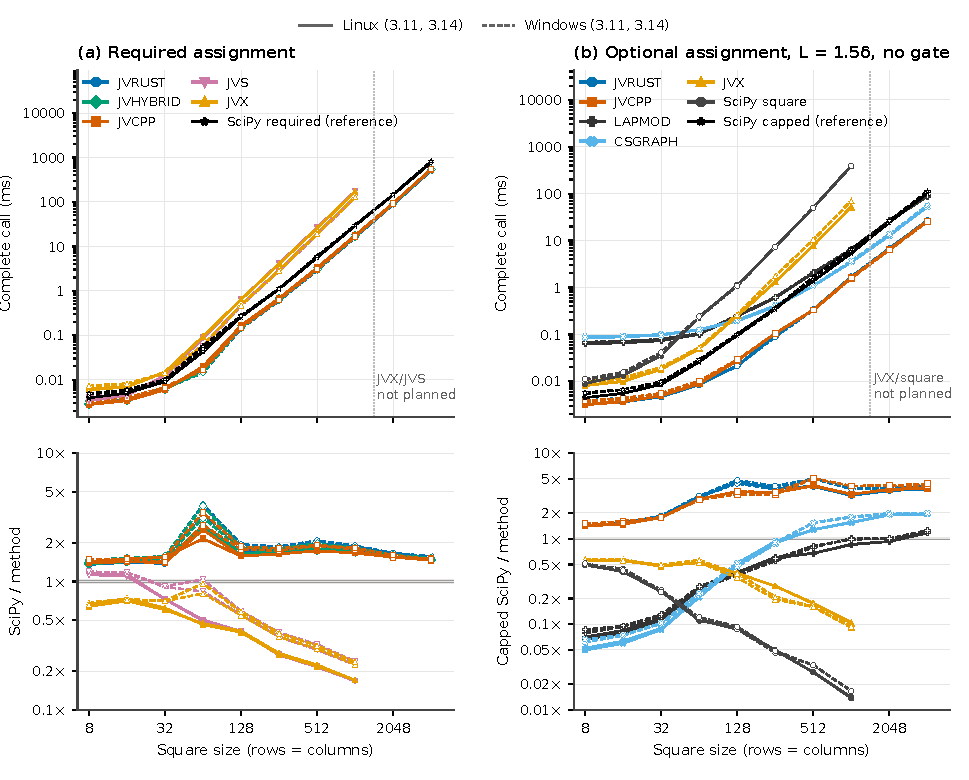
\includegraphics[width=\textwidth,height=.82\textheight,keepaspectratio]{images/current/S_geometry_lines_q06_square.pdf}
\end{center}
\clearpage
\section*{Atlas 2. Geometry: q=0.9, sd=0.25$\delta$, 5:4}
\noindent Ten saved sizes per objective. Runtime above, matching SciPy/method ratios below. Each curve is one method/environment. Only planned methods are connected; the light cutoff is marked.
\par\medskip
\begin{center}
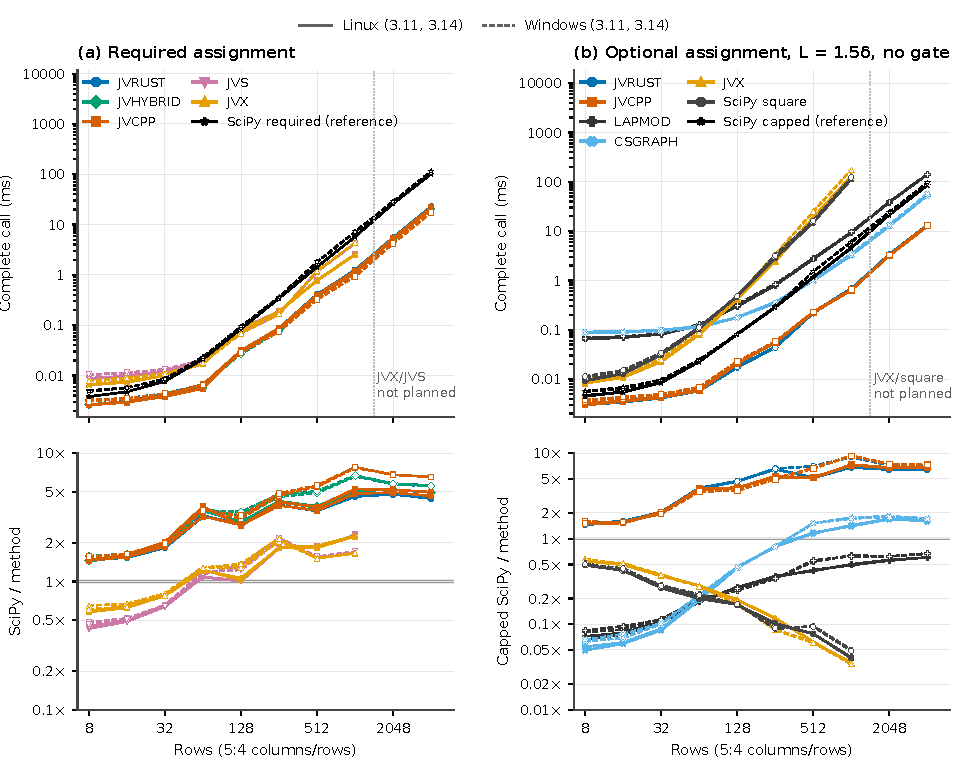
\includegraphics[width=\textwidth,height=.82\textheight,keepaspectratio]{images/current/S_geometry_lines_q09_5to4.pdf}
\end{center}
\clearpage
\section*{Atlas 3. Geometry: q=0.6, sd=1$\delta$, 5:4}
\noindent Ten saved sizes per objective. Runtime above, matching SciPy/method ratios below. Each curve is one method/environment. Only planned methods are connected; the light cutoff is marked.
\par\medskip
\begin{center}
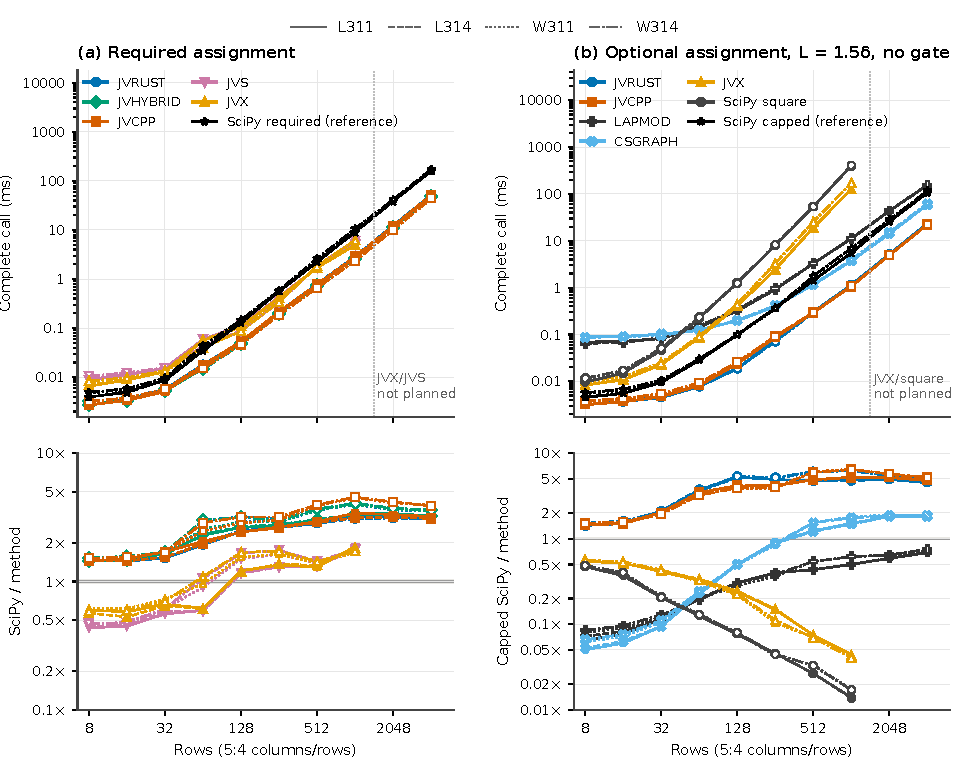
\includegraphics[width=\textwidth,height=.82\textheight,keepaspectratio]{images/current/S_geometry_lines_q06_5to4.pdf}
\end{center}
\clearpage
\section*{Atlas 4. Required square}
\noindent 7 saved sizes. Top: complete-call milliseconds. Bottom: matching SciPy/method ratio. Each curve is one method and one environment; OS encoding is solid/filled Linux and dashed/open Windows. Only planned observations are drawn. Exact values are in A1\_scaling.csv.
\par\medskip
\begin{center}
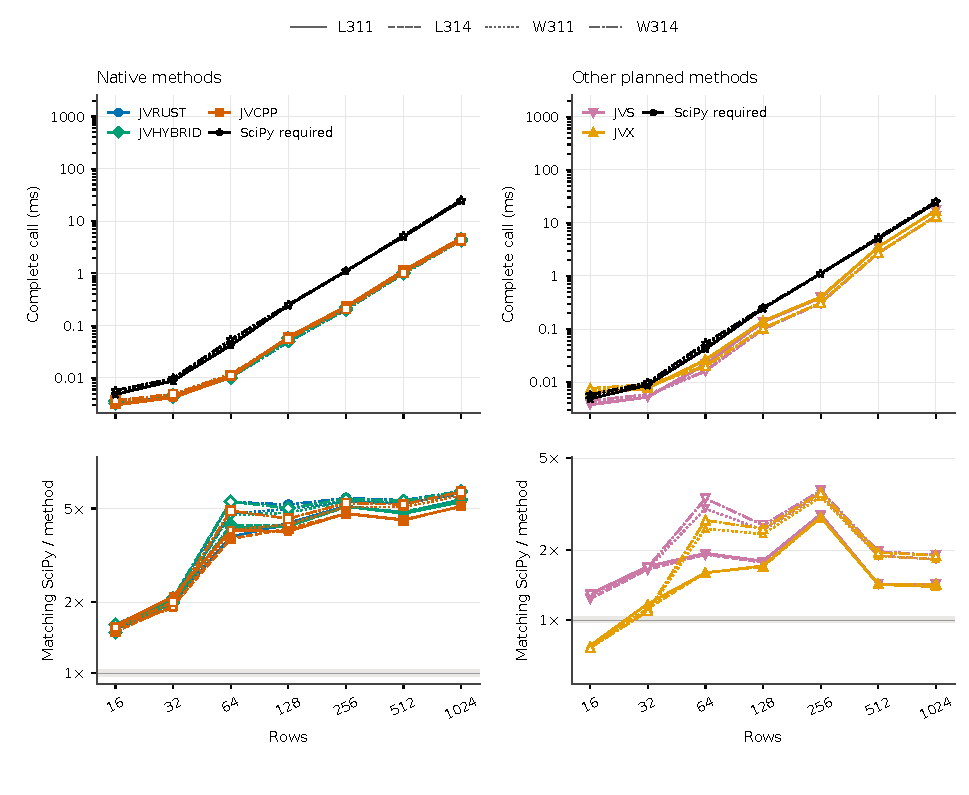
\includegraphics[width=\textwidth,height=.82\textheight,keepaspectratio]{images/current/S_scaling_lines_01.pdf}
\end{center}
\clearpage
\section*{Atlas 5. Required wide}
\noindent 6 saved sizes. Top: complete-call milliseconds. Bottom: matching SciPy/method ratio. Each curve is one method and one environment; OS encoding is solid/filled Linux and dashed/open Windows. Only planned observations are drawn. Exact values are in A1\_scaling.csv.
\par\medskip
\begin{center}
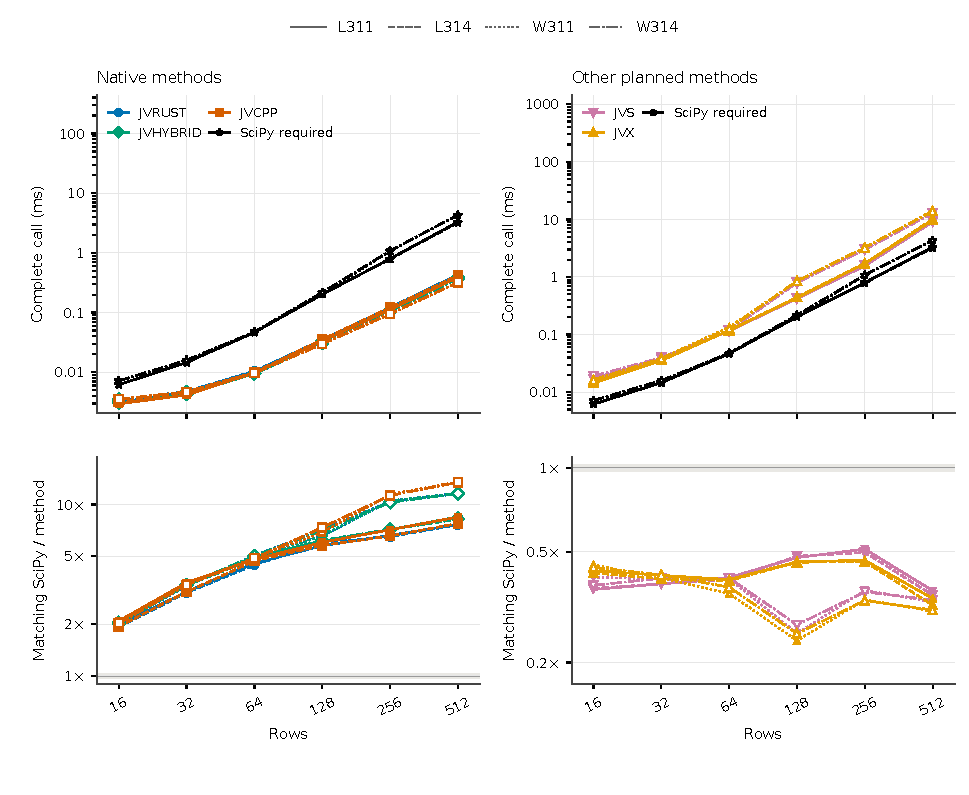
\includegraphics[width=\textwidth,height=.82\textheight,keepaspectratio]{images/current/S_scaling_lines_02.pdf}
\end{center}
\clearpage
\section*{Atlas 6. Required fixed}
\noindent 7 saved sizes. Top: complete-call milliseconds. Bottom: matching SciPy/method ratio. Each curve is one method and one environment; OS encoding is solid/filled Linux and dashed/open Windows. Only planned observations are drawn. Exact values are in A1\_scaling.csv.
\par\medskip
\begin{center}
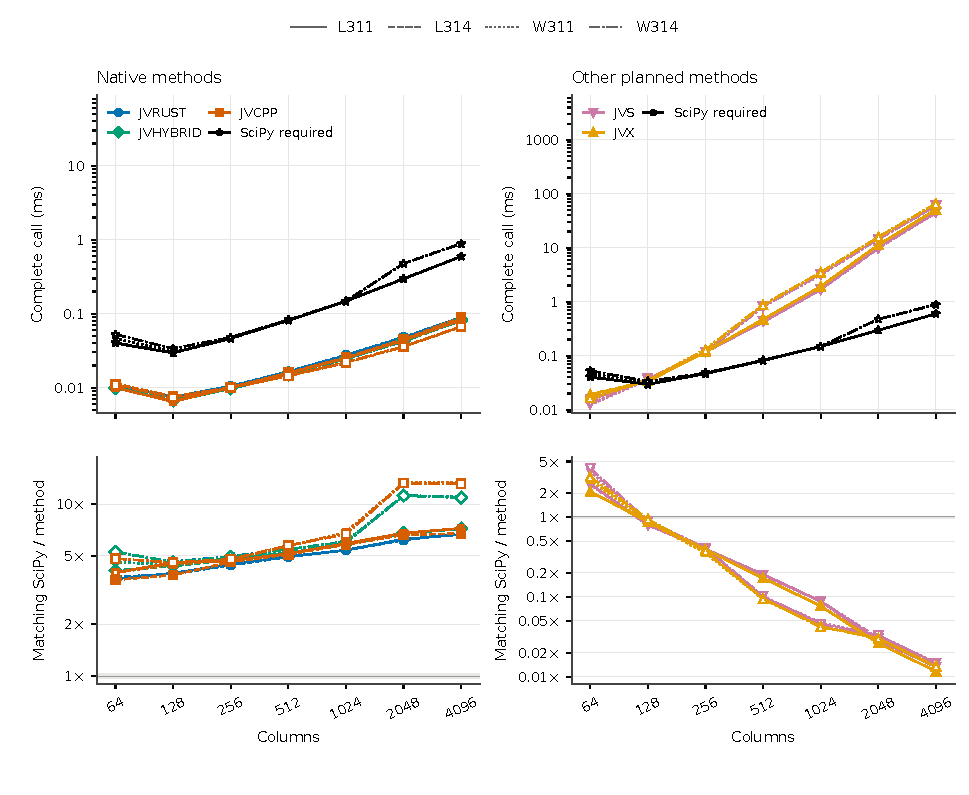
\includegraphics[width=\textwidth,height=.82\textheight,keepaspectratio]{images/current/S_scaling_lines_03.pdf}
\end{center}
\clearpage
\section*{Atlas 7. Optional square}
\noindent 7 saved sizes. Top: complete-call milliseconds. Bottom: matching SciPy/method ratio. Each curve is one method and one environment; OS encoding is solid/filled Linux and dashed/open Windows. Only planned observations are drawn. Exact values are in A1\_scaling.csv.
\par\medskip
\begin{center}
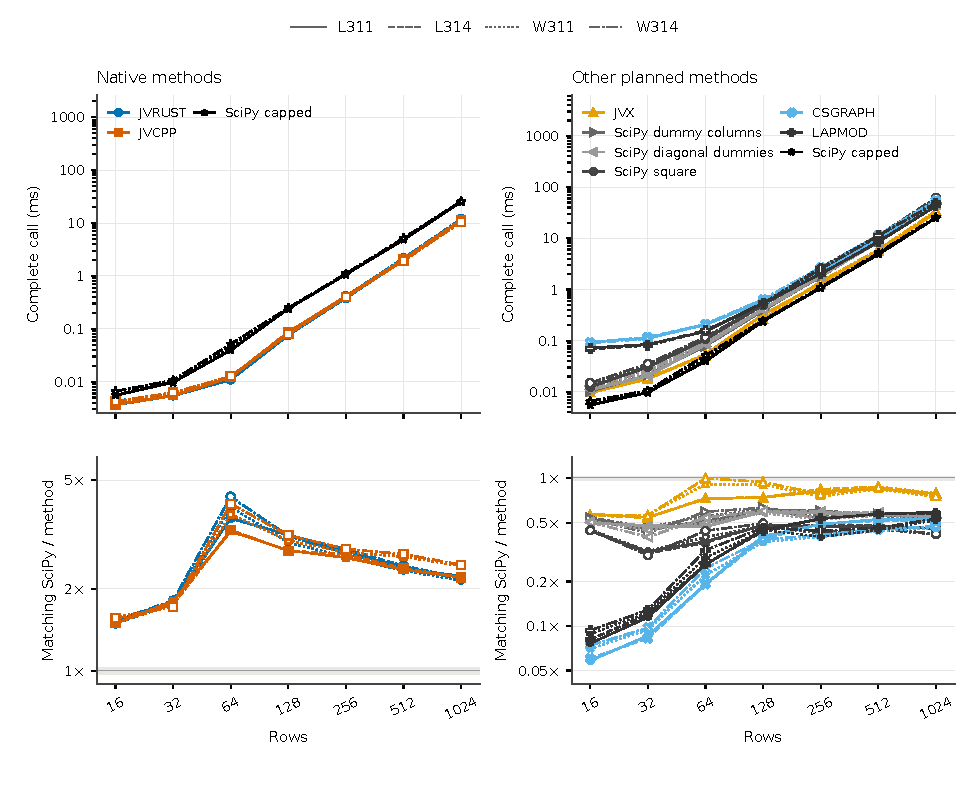
\includegraphics[width=\textwidth,height=.82\textheight,keepaspectratio]{images/current/S_scaling_lines_04.pdf}
\end{center}
\clearpage
\section*{Atlas 8. Optional wide}
\noindent 6 saved sizes. Top: complete-call milliseconds. Bottom: matching SciPy/method ratio. Each curve is one method and one environment; OS encoding is solid/filled Linux and dashed/open Windows. Only planned observations are drawn. Exact values are in A1\_scaling.csv.
\par\medskip
\begin{center}
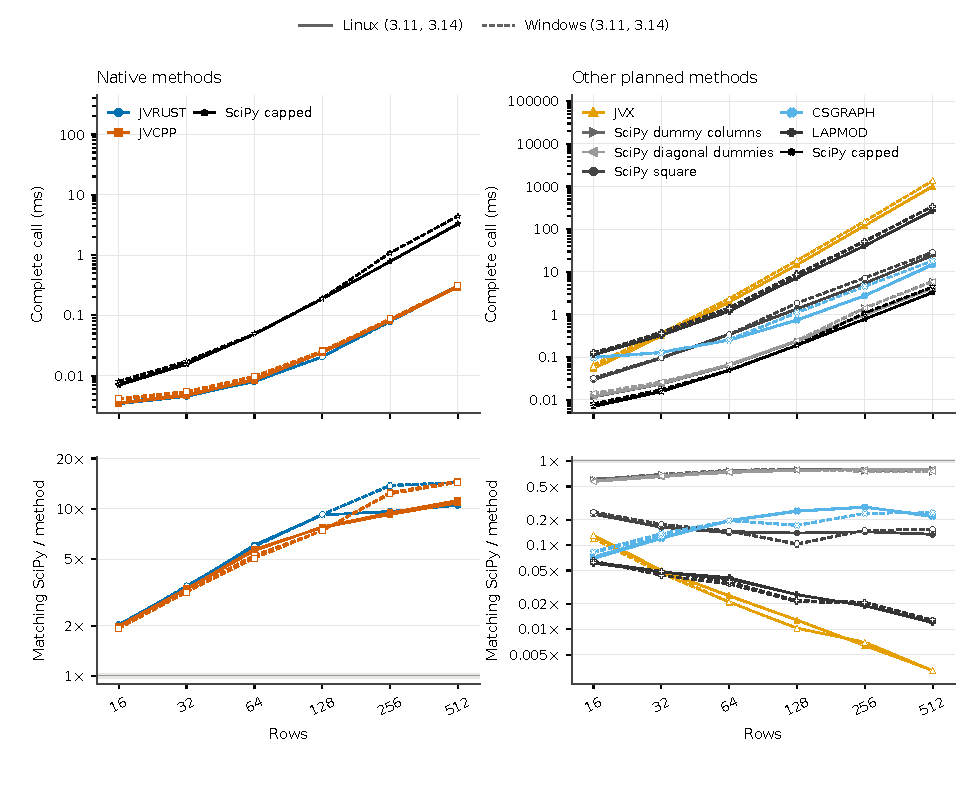
\includegraphics[width=\textwidth,height=.82\textheight,keepaspectratio]{images/current/S_scaling_lines_05.pdf}
\end{center}
\clearpage
\section*{Atlas 9. Optional fixed}
\noindent 7 saved sizes. Top: complete-call milliseconds. Bottom: matching SciPy/method ratio. Each curve is one method and one environment; OS encoding is solid/filled Linux and dashed/open Windows. Only planned observations are drawn. Exact values are in A1\_scaling.csv.
\par\medskip
\begin{center}
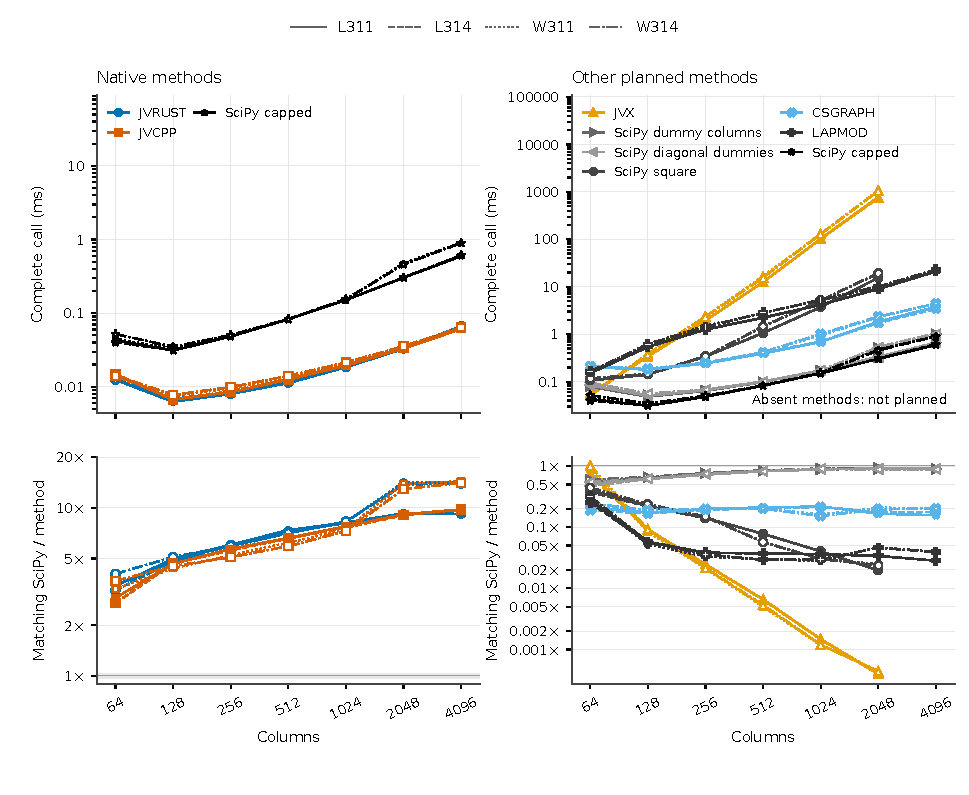
\includegraphics[width=\textwidth,height=.82\textheight,keepaspectratio]{images/current/S_scaling_lines_06.pdf}
\end{center}
\clearpage
\section*{Atlas 10. Optional blocks}
\noindent 7 saved sizes. Top: complete-call milliseconds. Bottom: matching SciPy/method ratio. Each curve is one method and one environment; OS encoding is solid/filled Linux and dashed/open Windows. Only planned observations are drawn. Exact values are in A1\_scaling.csv.
\par\medskip
\begin{center}
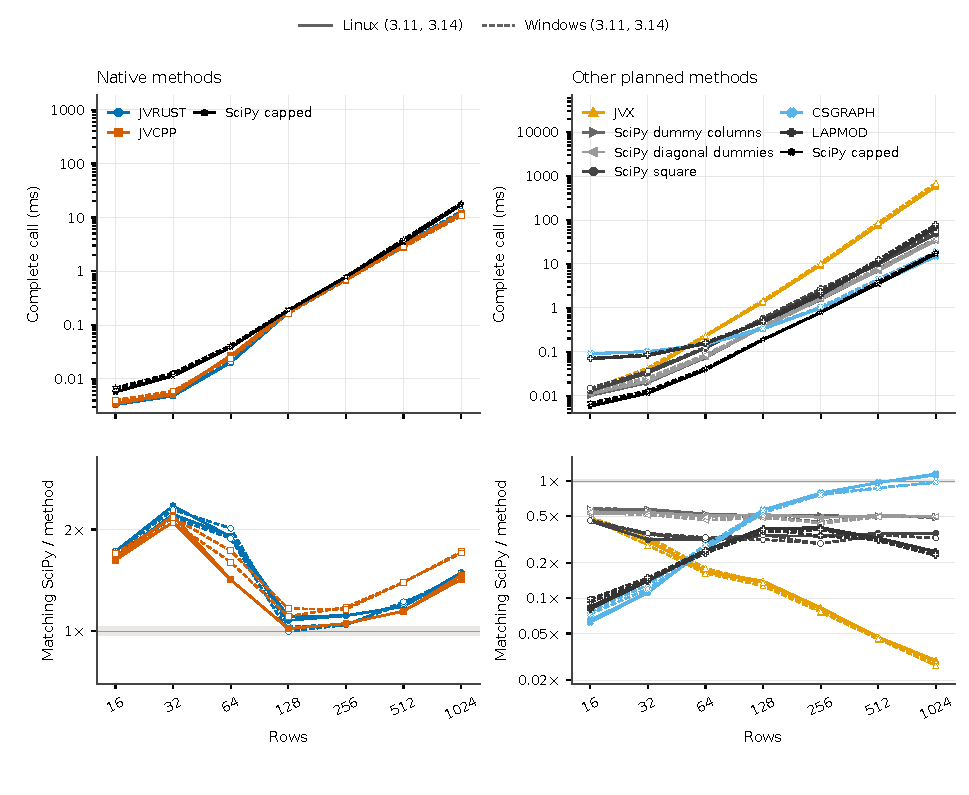
\includegraphics[width=\textwidth,height=.82\textheight,keepaspectratio]{images/current/S_scaling_lines_07.pdf}
\end{center}
\clearpage
\section*{Atlas 11. Large square required}
\noindent 4 saved sizes. Top: complete-call milliseconds. Bottom: matching SciPy/method ratio. Each curve is one method and one environment; OS encoding is solid/filled Linux and dashed/open Windows. Only planned observations are drawn. Exact values are in A1\_scaling.csv.
\par\medskip
\begin{center}
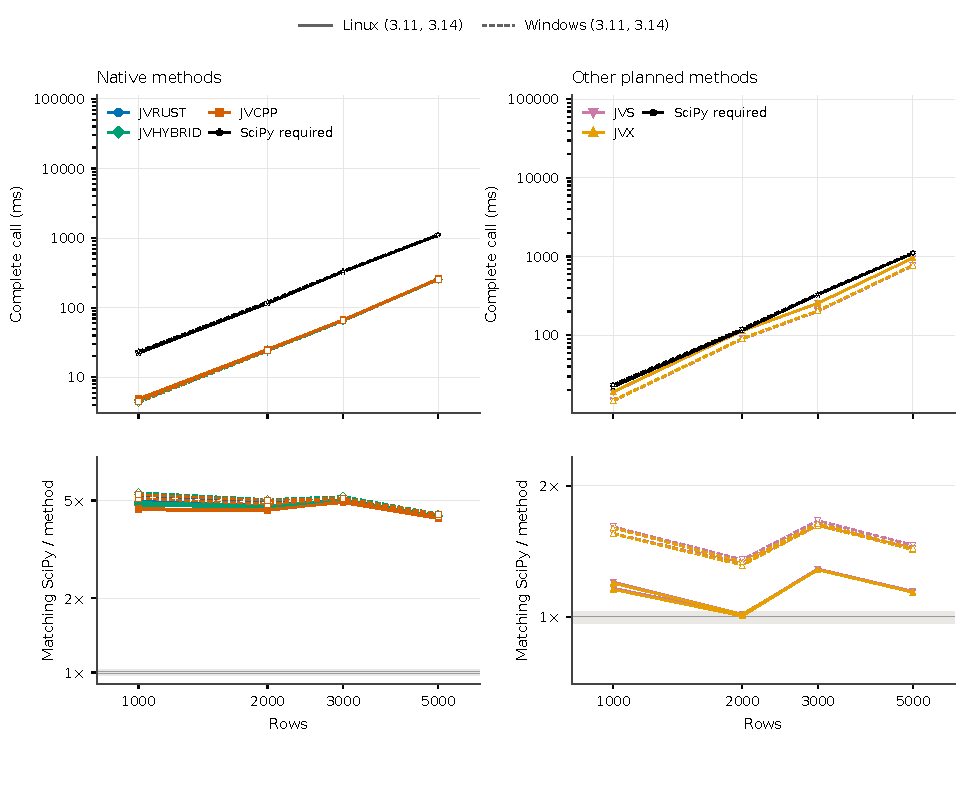
\includegraphics[width=\textwidth,height=.82\textheight,keepaspectratio]{images/current/S_scaling_lines_08.pdf}
\end{center}
\clearpage
\section*{Atlas 12. Large square optional}
\noindent 4 saved sizes. Top: complete-call milliseconds. Bottom: matching SciPy/method ratio. Each curve is one method and one environment; OS encoding is solid/filled Linux and dashed/open Windows. Only planned observations are drawn. Exact values are in A1\_scaling.csv.
\par\medskip
\begin{center}
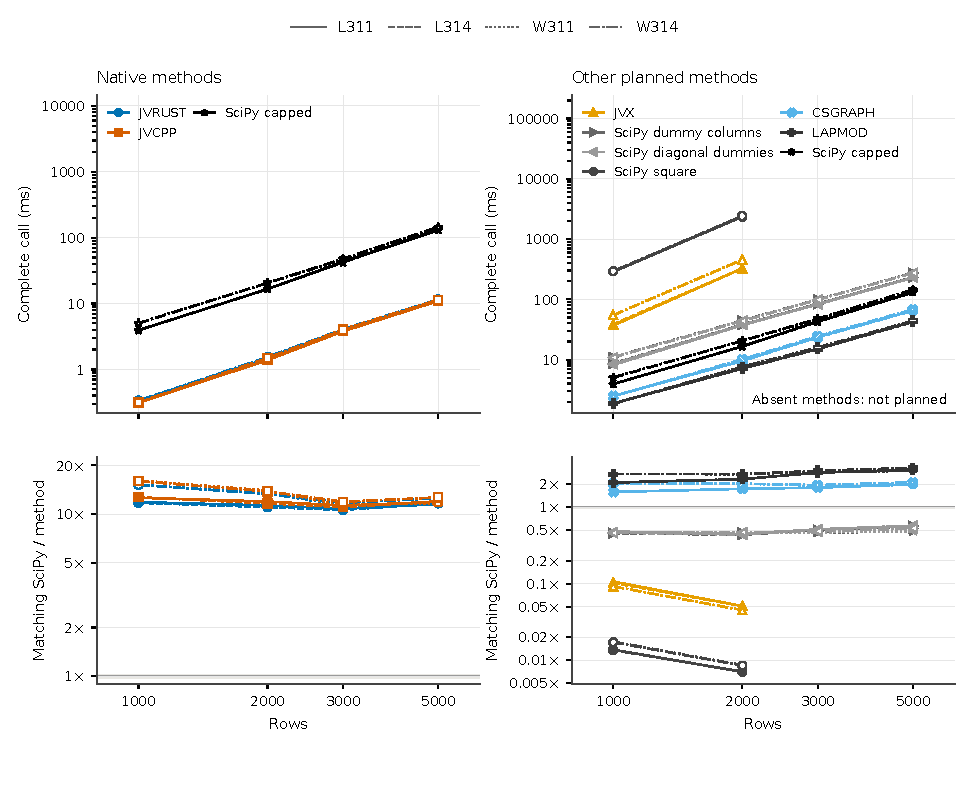
\includegraphics[width=\textwidth,height=.82\textheight,keepaspectratio]{images/current/S_scaling_lines_09.pdf}
\end{center}
\clearpage
\section*{Atlas 13. Large rectangle required wide}
\noindent 3 saved sizes. Top: complete-call milliseconds. Bottom: matching SciPy/method ratio. Each curve is one method and one environment; OS encoding is solid/filled Linux and dashed/open Windows. Only planned observations are drawn. Exact values are in A1\_scaling.csv.
\par\medskip
\begin{center}
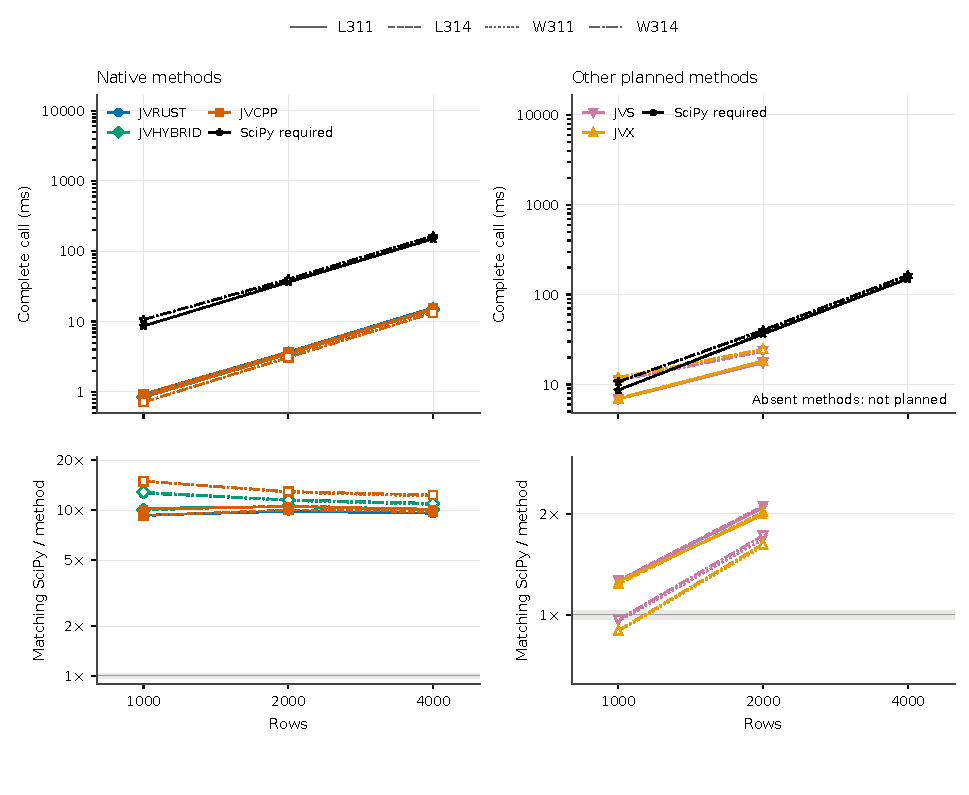
\includegraphics[width=\textwidth,height=.82\textheight,keepaspectratio]{images/current/S_scaling_lines_10.pdf}
\end{center}
\clearpage
\section*{Atlas 14. Large rectangle optional wide}
\noindent 3 saved sizes. Top: complete-call milliseconds. Bottom: matching SciPy/method ratio. Each curve is one method and one environment; OS encoding is solid/filled Linux and dashed/open Windows. Only planned observations are drawn. Exact values are in A1\_scaling.csv.
\par\medskip
\begin{center}
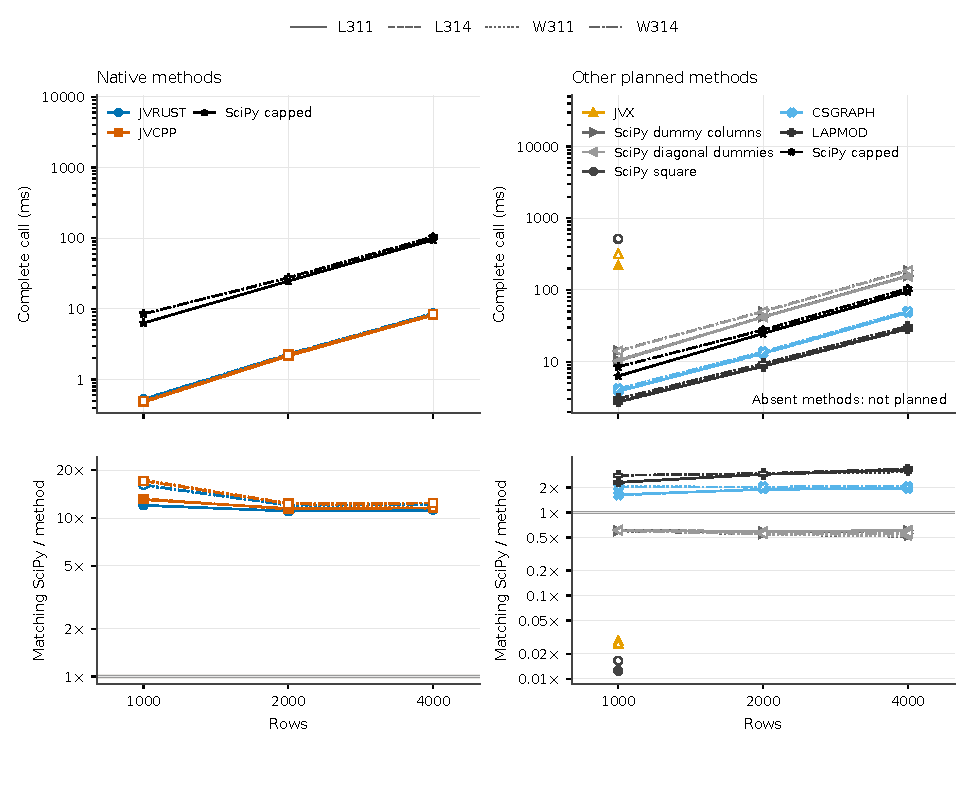
\includegraphics[width=\textwidth,height=.82\textheight,keepaspectratio]{images/current/S_scaling_lines_11.pdf}
\end{center}
\clearpage
\section*{Atlas 15. Large rectangle required tall}
\noindent 3 saved sizes. Top: complete-call milliseconds. Bottom: matching SciPy/method ratio. Each curve is one method and one environment; OS encoding is solid/filled Linux and dashed/open Windows. Only planned observations are drawn. Exact values are in A1\_scaling.csv.
\par\medskip
\begin{center}
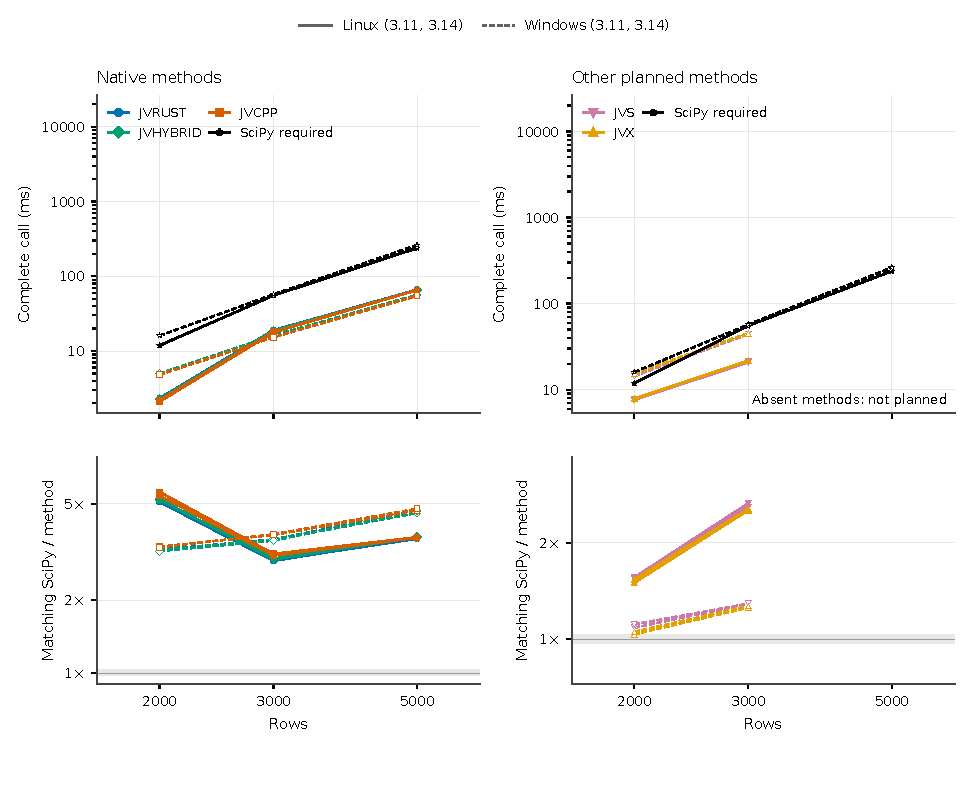
\includegraphics[width=\textwidth,height=.82\textheight,keepaspectratio]{images/current/S_scaling_lines_12.pdf}
\end{center}
\clearpage
\section*{Atlas 16. Large rectangle optional tall}
\noindent 3 saved sizes. Top: complete-call milliseconds. Bottom: matching SciPy/method ratio. Each curve is one method and one environment; OS encoding is solid/filled Linux and dashed/open Windows. Only planned observations are drawn. Exact values are in A1\_scaling.csv.
\par\medskip
\begin{center}
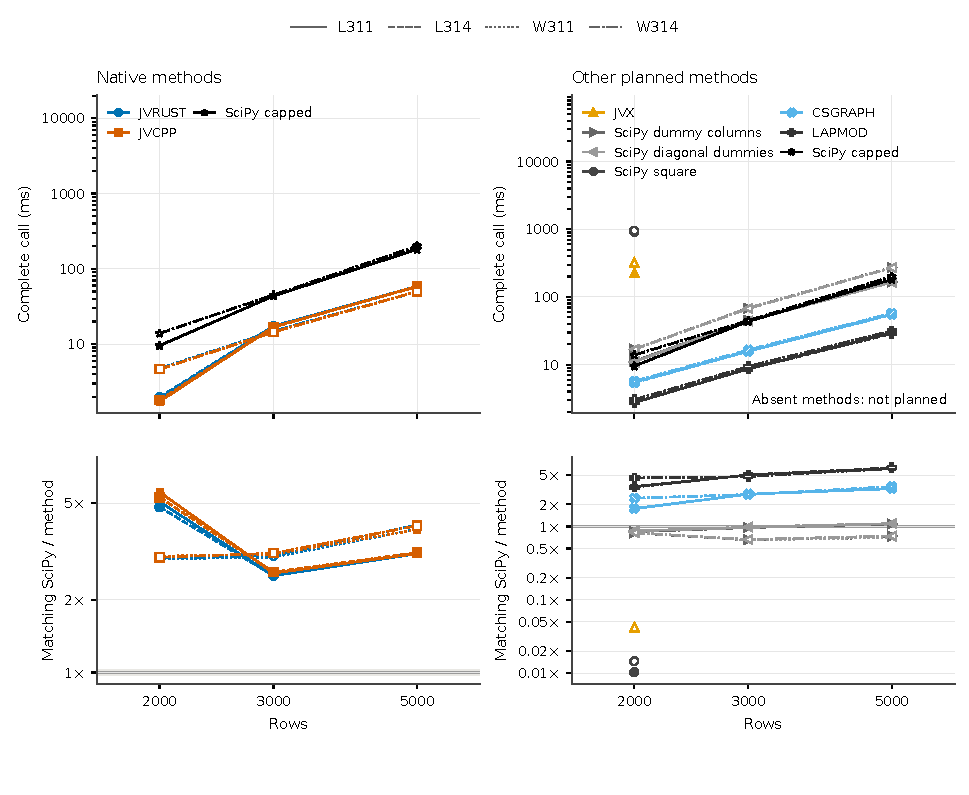
\includegraphics[width=\textwidth,height=.82\textheight,keepaspectratio]{images/current/S_scaling_lines_13.pdf}
\end{center}
\clearpage
\section*{Atlas 17. Extreme rectangle required wide}
\noindent 3 saved sizes. Top: complete-call milliseconds. Bottom: matching SciPy/method ratio. Each curve is one method and one environment; OS encoding is solid/filled Linux and dashed/open Windows. Only planned observations are drawn. Exact values are in A1\_scaling.csv.
\par\medskip
\begin{center}
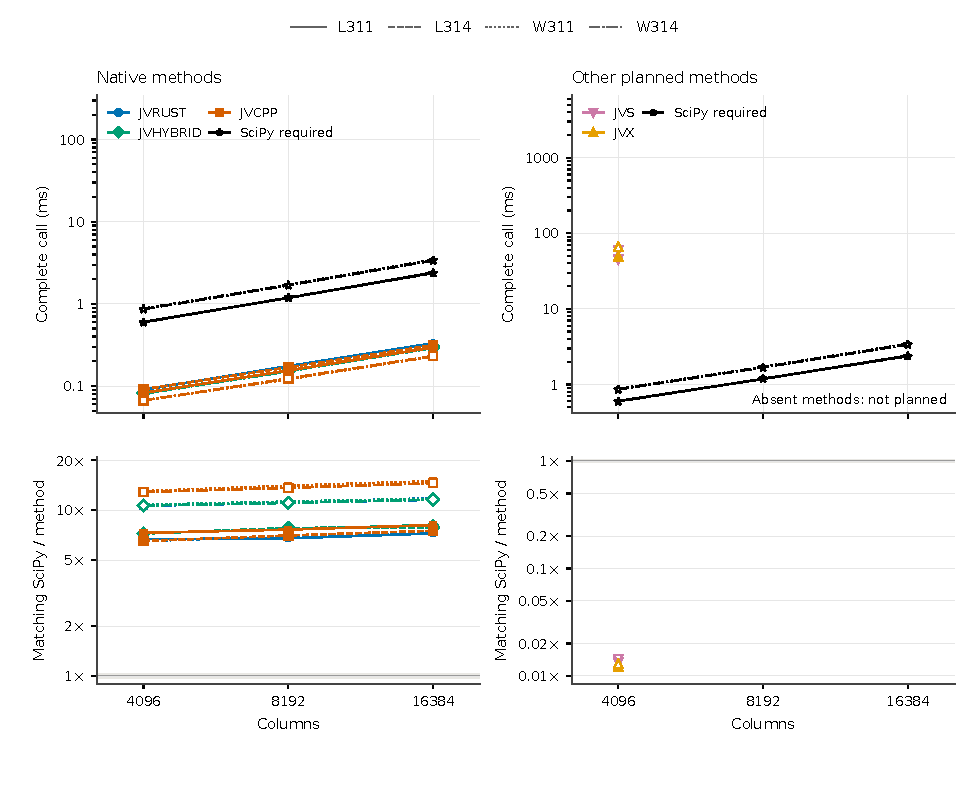
\includegraphics[width=\textwidth,height=.82\textheight,keepaspectratio]{images/current/S_scaling_lines_14.pdf}
\end{center}
\clearpage
\section*{Atlas 18. Extreme rectangle optional wide}
\noindent 3 saved sizes. Top: complete-call milliseconds. Bottom: matching SciPy/method ratio. Each curve is one method and one environment; OS encoding is solid/filled Linux and dashed/open Windows. Only planned observations are drawn. Exact values are in A1\_scaling.csv.
\par\medskip
\begin{center}
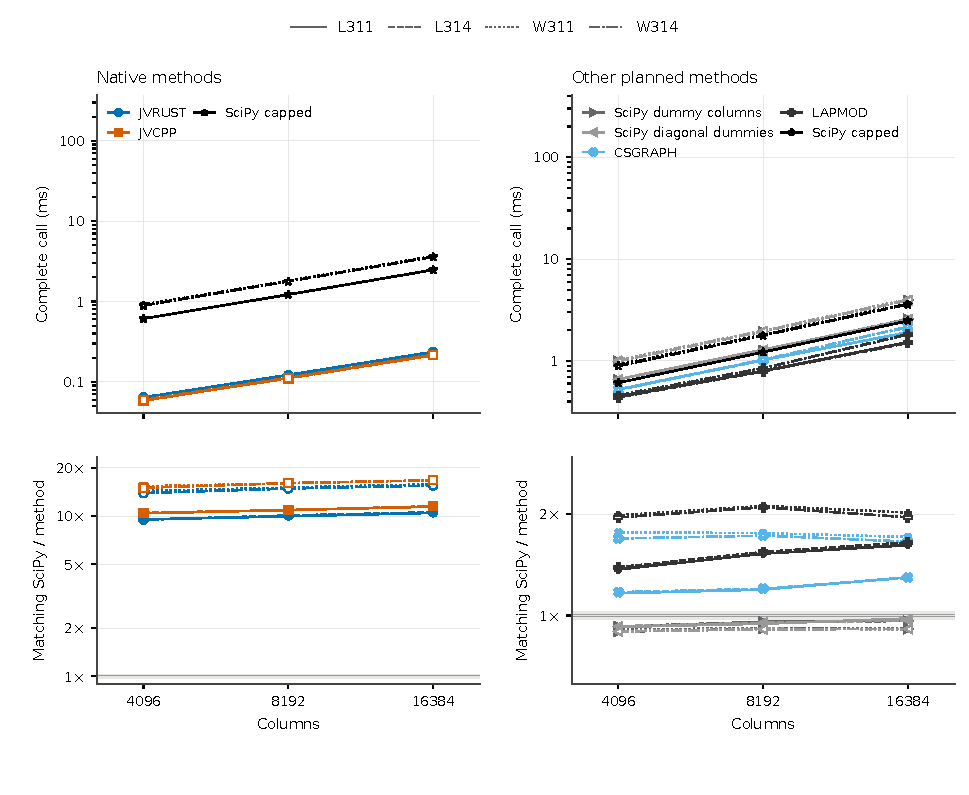
\includegraphics[width=\textwidth,height=.82\textheight,keepaspectratio]{images/current/S_scaling_lines_15.pdf}
\end{center}
\clearpage
\section*{Atlas 19. Extreme rectangle required tall}
\noindent 3 saved sizes. Top: complete-call milliseconds. Bottom: matching SciPy/method ratio. Each curve is one method and one environment; OS encoding is solid/filled Linux and dashed/open Windows. Only planned observations are drawn. Exact values are in A1\_scaling.csv.
\par\medskip
\begin{center}
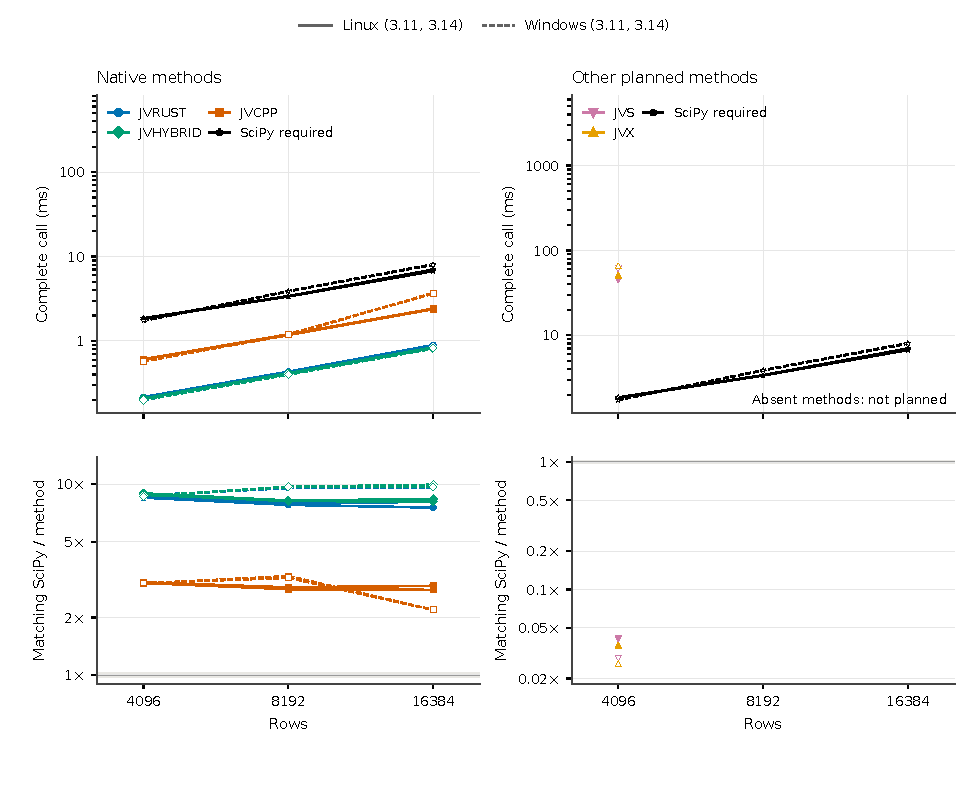
\includegraphics[width=\textwidth,height=.82\textheight,keepaspectratio]{images/current/S_scaling_lines_16.pdf}
\end{center}
\clearpage
\section*{Atlas 20. Extreme rectangle optional tall}
\noindent 3 saved sizes. Top: complete-call milliseconds. Bottom: matching SciPy/method ratio. Each curve is one method and one environment; OS encoding is solid/filled Linux and dashed/open Windows. Only planned observations are drawn. Exact values are in A1\_scaling.csv.
\par\medskip
\begin{center}
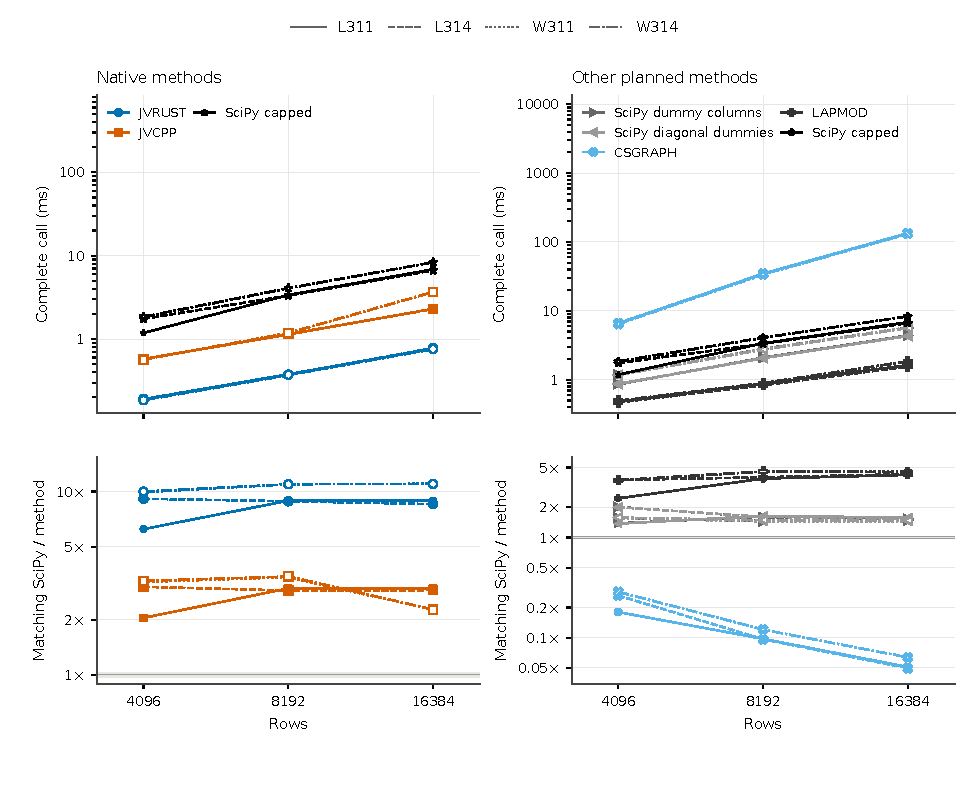
\includegraphics[width=\textwidth,height=.82\textheight,keepaspectratio]{images/current/S_scaling_lines_17.pdf}
\end{center}
\clearpage
\section*{Atlas 21. Rust policy cases, page 1/8}
\noindent One row per workload; R/O mean required/optional. Left: the ordered reduction-budget sweep. Right: independent nominal interventions, drawn only where planned. Every mark/curve is one environment. Ratios are intervention/reference, so above one is slower. Exact case identities and all values remain in the indexed S3 policy timing exports and F5\_budget\_data.csv.
\par\medskip
\begin{center}
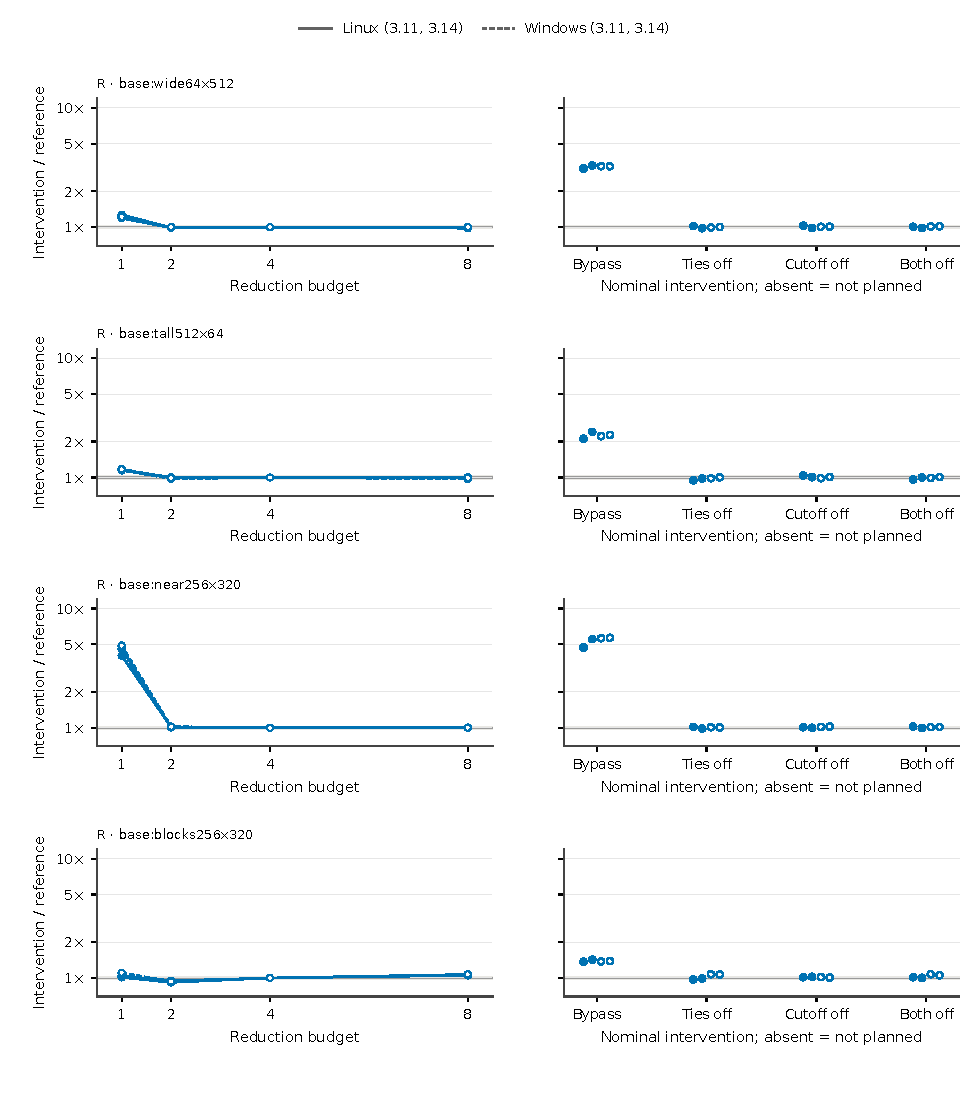
\includegraphics[width=\textwidth,height=.82\textheight,keepaspectratio]{images/current/S_policy_lines_rust_1.pdf}
\end{center}
\clearpage
\section*{Atlas 22. Rust policy cases, page 2/8}
\noindent One row per workload; R/O mean required/optional. Left: the ordered reduction-budget sweep. Right: independent nominal interventions, drawn only where planned. Every mark/curve is one environment. Ratios are intervention/reference, so above one is slower. Exact case identities and all values remain in the indexed S3 policy timing exports and F5\_budget\_data.csv.
\par\medskip
\begin{center}
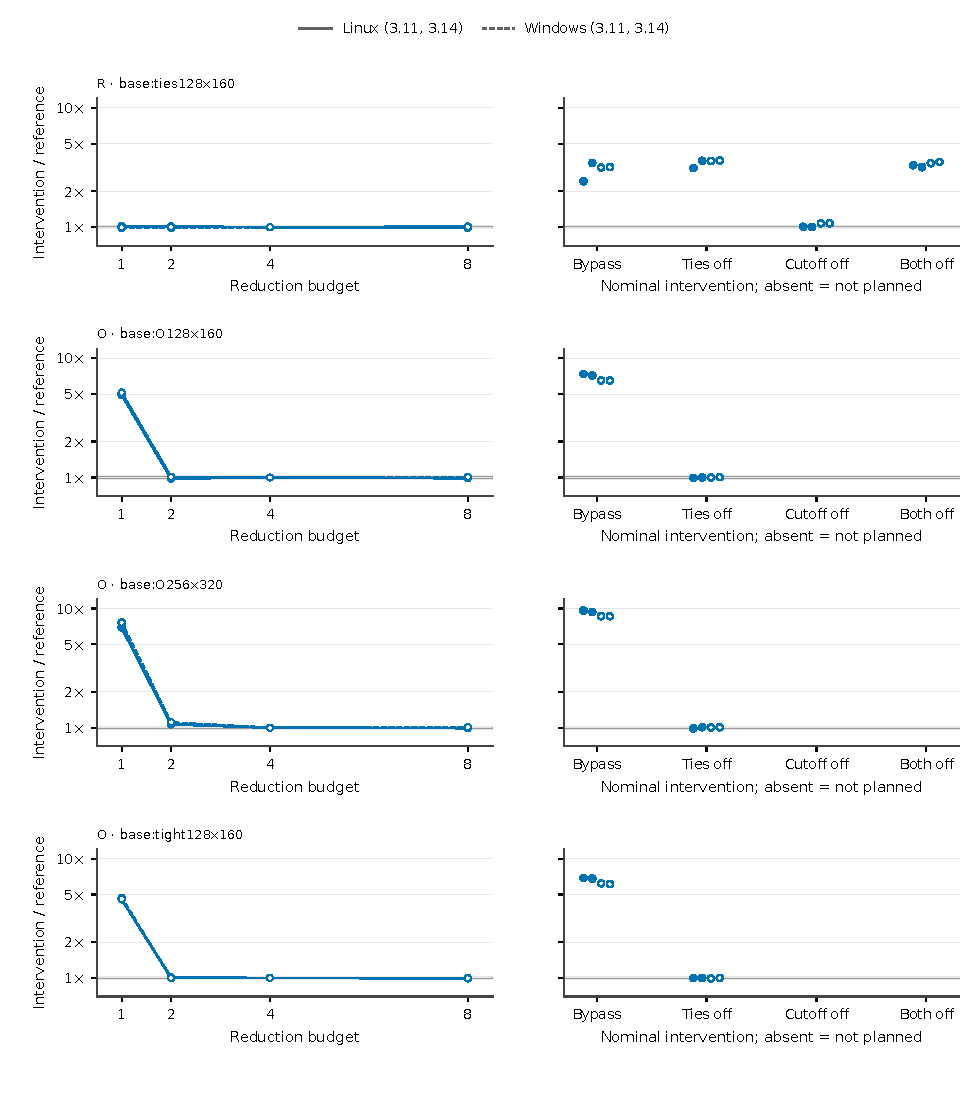
\includegraphics[width=\textwidth,height=.82\textheight,keepaspectratio]{images/current/S_policy_lines_rust_2.pdf}
\end{center}
\clearpage
\section*{Atlas 23. Rust policy cases, page 3/8}
\noindent One row per workload; R/O mean required/optional. Left: the ordered reduction-budget sweep. Right: independent nominal interventions, drawn only where planned. Every mark/curve is one environment. Ratios are intervention/reference, so above one is slower. Exact case identities and all values remain in the indexed S3 policy timing exports and F5\_budget\_data.csv.
\par\medskip
\begin{center}
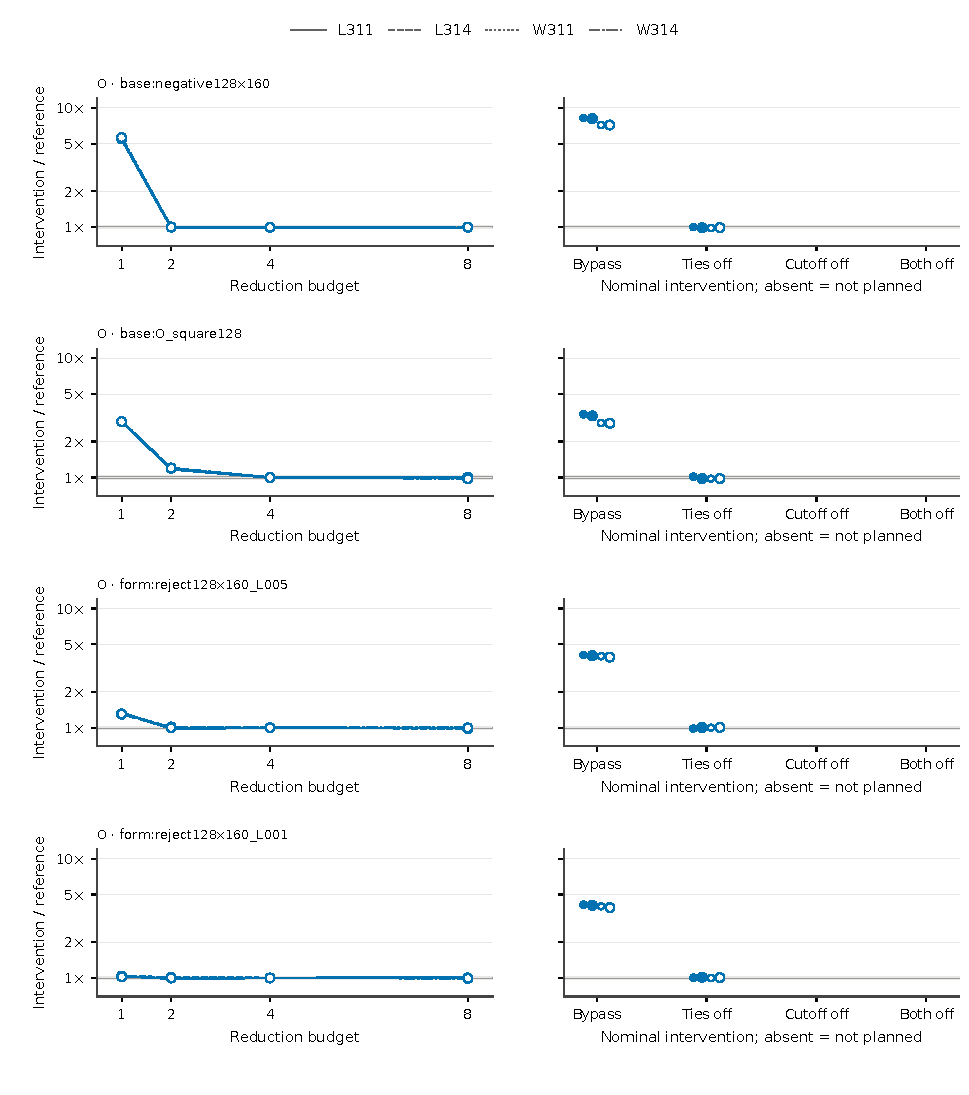
\includegraphics[width=\textwidth,height=.82\textheight,keepaspectratio]{images/current/S_policy_lines_rust_3.pdf}
\end{center}
\clearpage
\section*{Atlas 24. Rust policy cases, page 4/8}
\noindent One row per workload; R/O mean required/optional. Left: the ordered reduction-budget sweep. Right: independent nominal interventions, drawn only where planned. Every mark/curve is one environment. Ratios are intervention/reference, so above one is slower. Exact case identities and all values remain in the indexed S3 policy timing exports and F5\_budget\_data.csv.
\par\medskip
\begin{center}
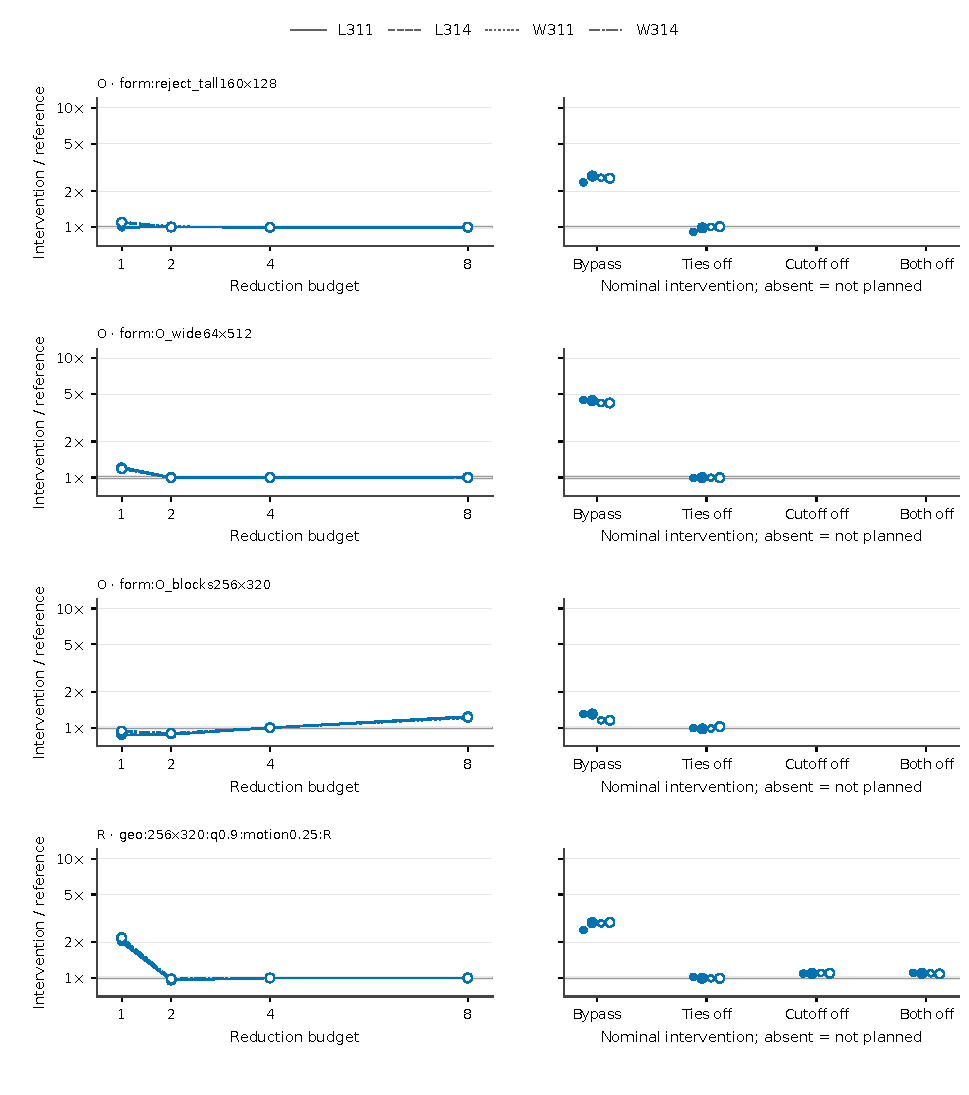
\includegraphics[width=\textwidth,height=.82\textheight,keepaspectratio]{images/current/S_policy_lines_rust_4.pdf}
\end{center}
\clearpage
\section*{Atlas 25. Rust policy cases, page 5/8}
\noindent One row per workload; R/O mean required/optional. Left: the ordered reduction-budget sweep. Right: independent nominal interventions, drawn only where planned. Every mark/curve is one environment. Ratios are intervention/reference, so above one is slower. Exact case identities and all values remain in the indexed S3 policy timing exports and F5\_budget\_data.csv.
\par\medskip
\begin{center}
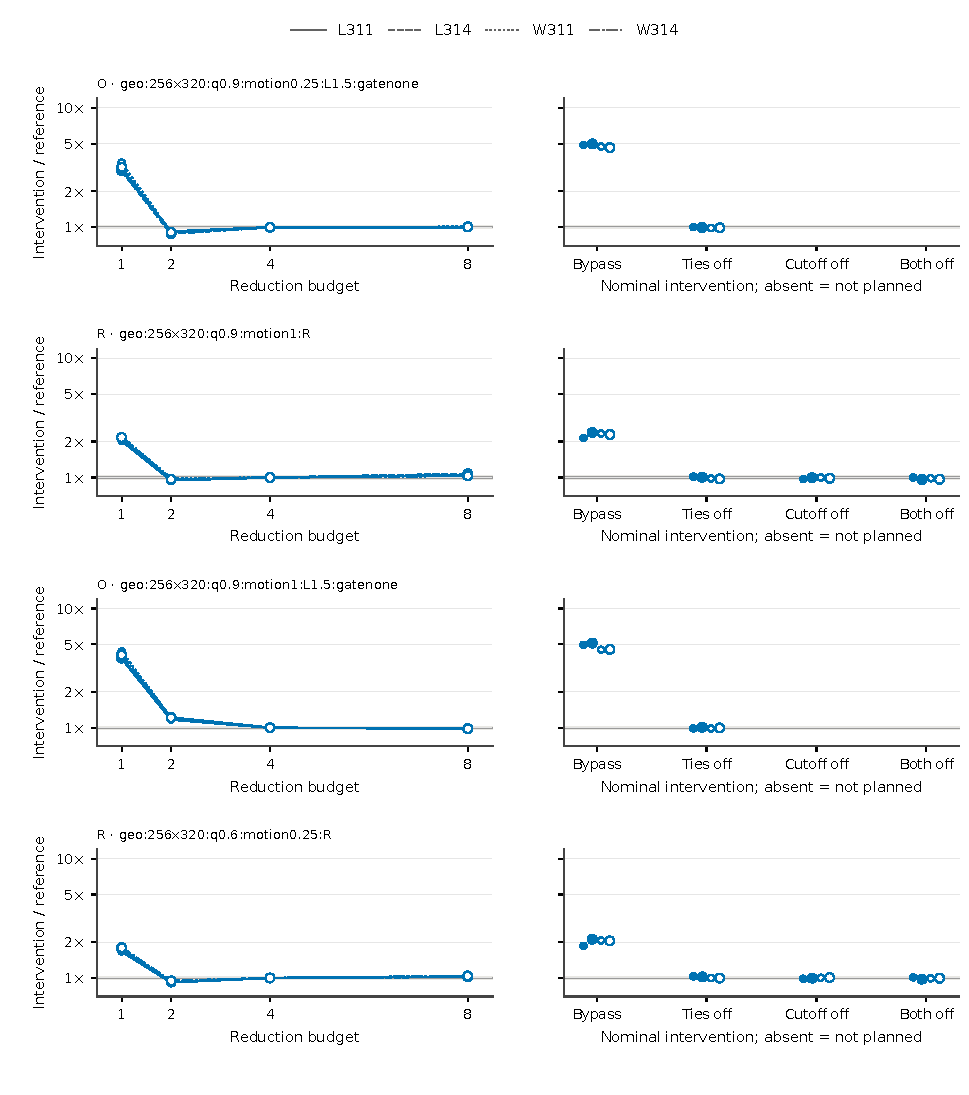
\includegraphics[width=\textwidth,height=.82\textheight,keepaspectratio]{images/current/S_policy_lines_rust_5.pdf}
\end{center}
\clearpage
\section*{Atlas 26. Rust policy cases, page 6/8}
\noindent One row per workload; R/O mean required/optional. Left: the ordered reduction-budget sweep. Right: independent nominal interventions, drawn only where planned. Every mark/curve is one environment. Ratios are intervention/reference, so above one is slower. Exact case identities and all values remain in the indexed S3 policy timing exports and F5\_budget\_data.csv.
\par\medskip
\begin{center}
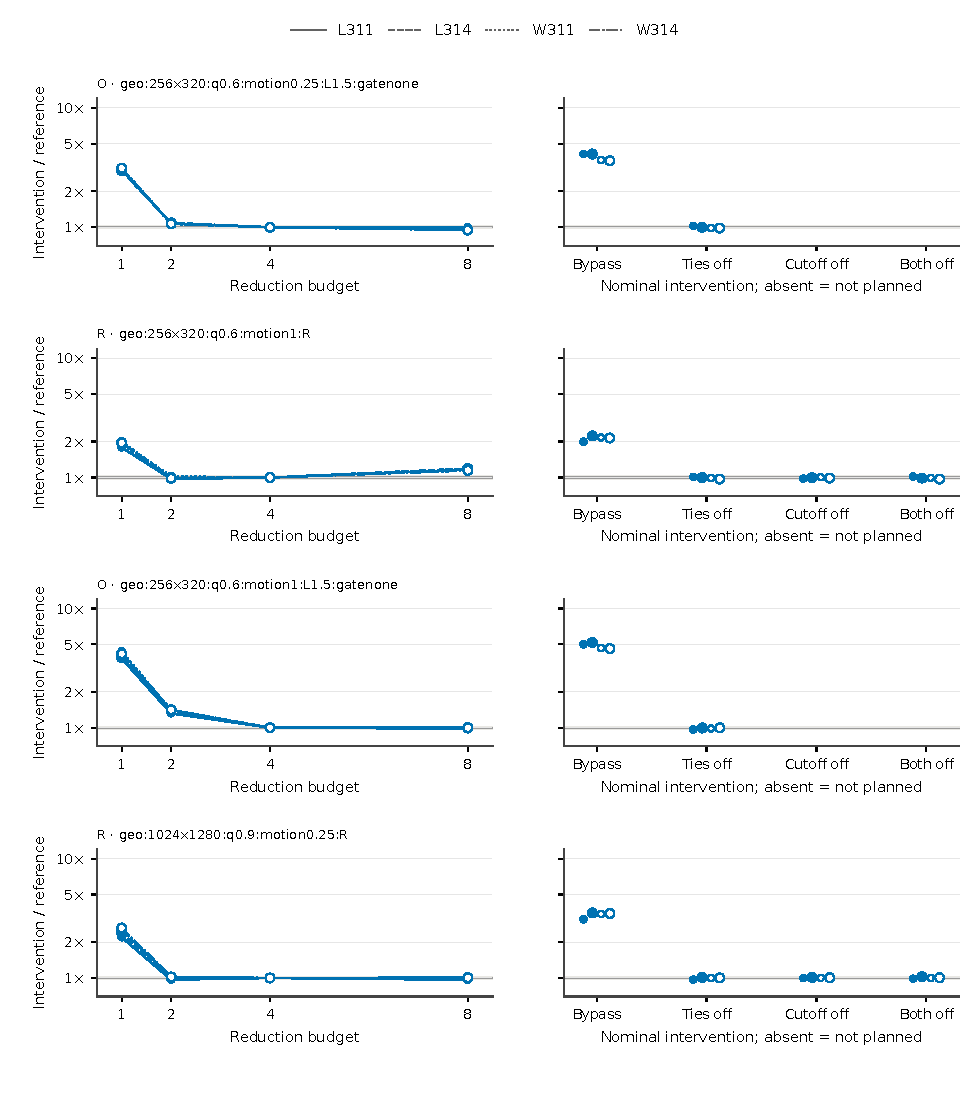
\includegraphics[width=\textwidth,height=.82\textheight,keepaspectratio]{images/current/S_policy_lines_rust_6.pdf}
\end{center}
\clearpage
\section*{Atlas 27. Rust policy cases, page 7/8}
\noindent One row per workload; R/O mean required/optional. Left: the ordered reduction-budget sweep. Right: independent nominal interventions, drawn only where planned. Every mark/curve is one environment. Ratios are intervention/reference, so above one is slower. Exact case identities and all values remain in the indexed S3 policy timing exports and F5\_budget\_data.csv.
\par\medskip
\begin{center}
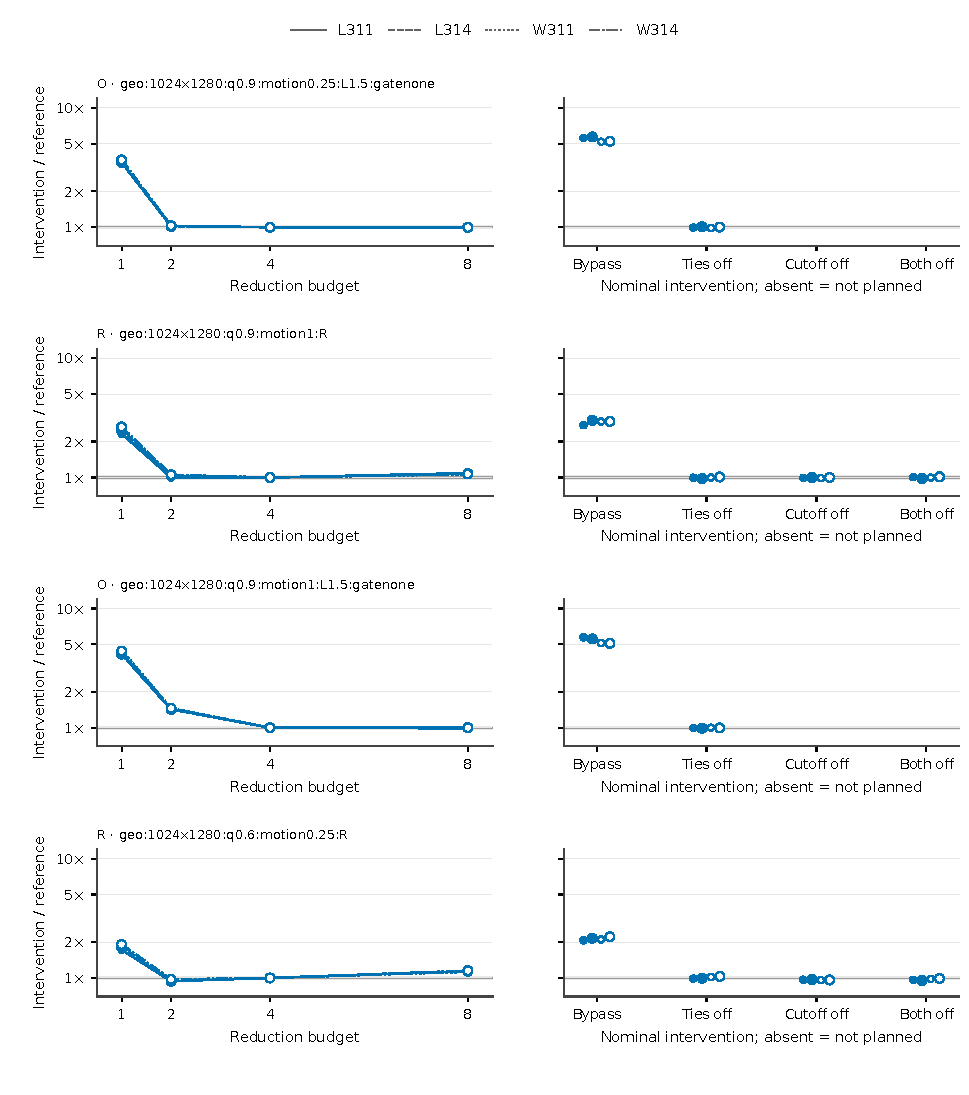
\includegraphics[width=\textwidth,height=.82\textheight,keepaspectratio]{images/current/S_policy_lines_rust_7.pdf}
\end{center}
\clearpage
\section*{Atlas 28. Rust policy cases, page 8/8}
\noindent One row per workload; R/O mean required/optional. Left: the ordered reduction-budget sweep. Right: independent nominal interventions, drawn only where planned. Every mark/curve is one environment. Ratios are intervention/reference, so above one is slower. Exact case identities and all values remain in the indexed S3 policy timing exports and F5\_budget\_data.csv.
\par\medskip
\begin{center}
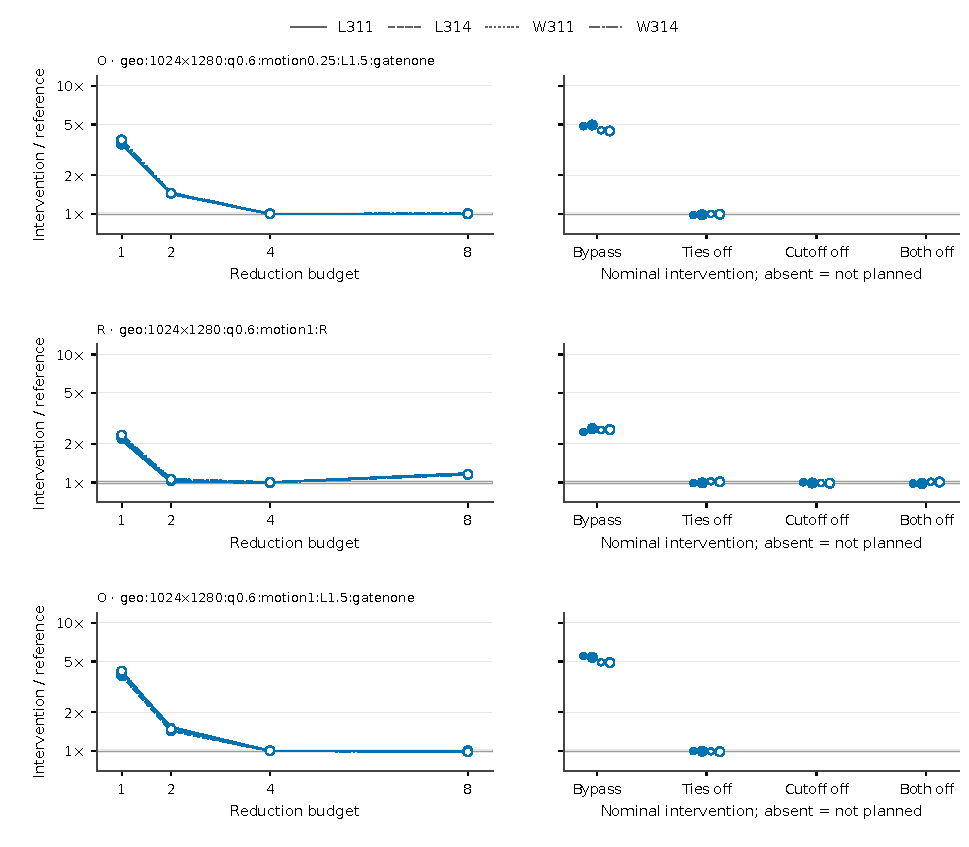
\includegraphics[width=\textwidth,height=.82\textheight,keepaspectratio]{images/current/S_policy_lines_rust_8.pdf}
\end{center}
\clearpage
\section*{Atlas 29. CPP policy cases, page 1/8}
\noindent One row per workload; R/O mean required/optional. Left: the ordered reduction-budget sweep. Right: independent nominal interventions, drawn only where planned. Every mark/curve is one environment. Ratios are intervention/reference, so above one is slower. Exact case identities and all values remain in the indexed S3 policy timing exports and F5\_budget\_data.csv.
\par\medskip
\begin{center}
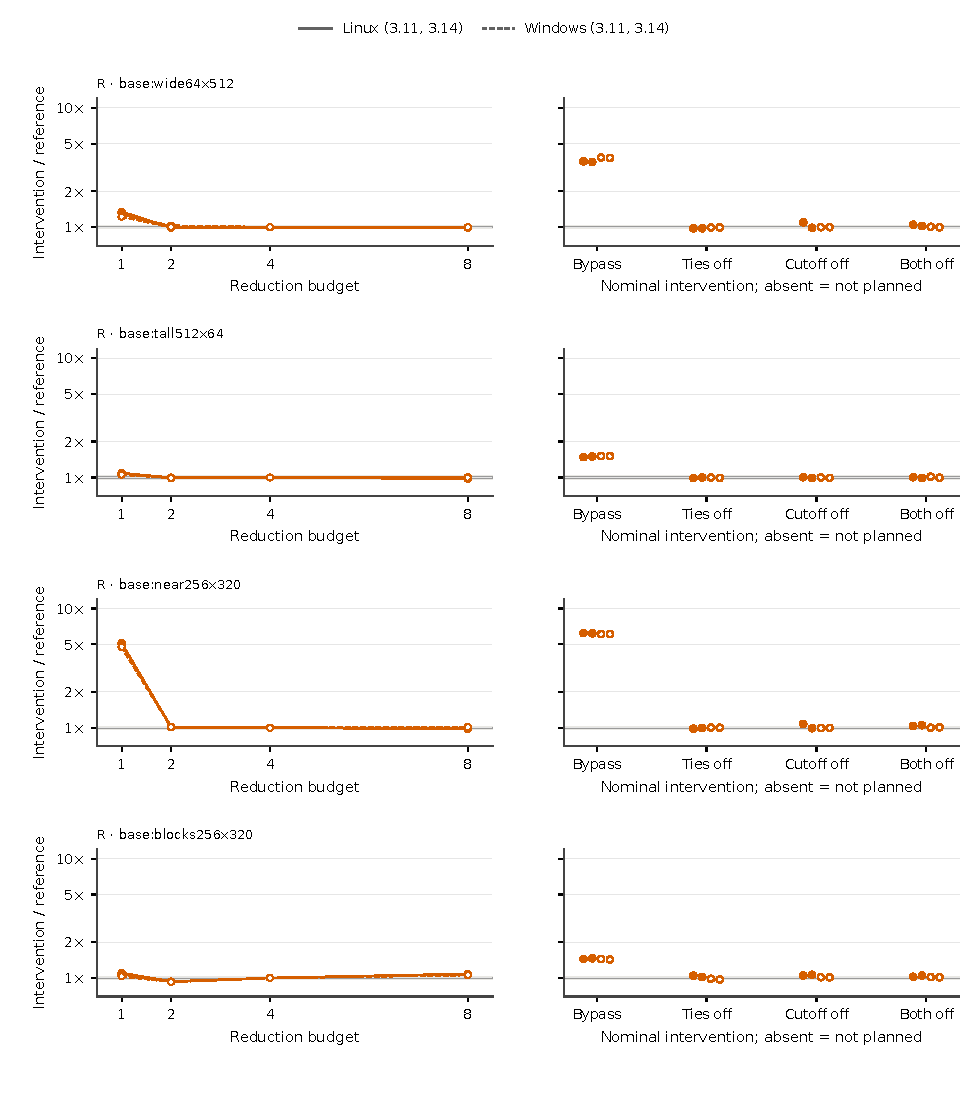
\includegraphics[width=\textwidth,height=.82\textheight,keepaspectratio]{images/current/S_policy_lines_cpp_1.pdf}
\end{center}
\clearpage
\section*{Atlas 30. CPP policy cases, page 2/8}
\noindent One row per workload; R/O mean required/optional. Left: the ordered reduction-budget sweep. Right: independent nominal interventions, drawn only where planned. Every mark/curve is one environment. Ratios are intervention/reference, so above one is slower. Exact case identities and all values remain in the indexed S3 policy timing exports and F5\_budget\_data.csv.
\par\medskip
\begin{center}
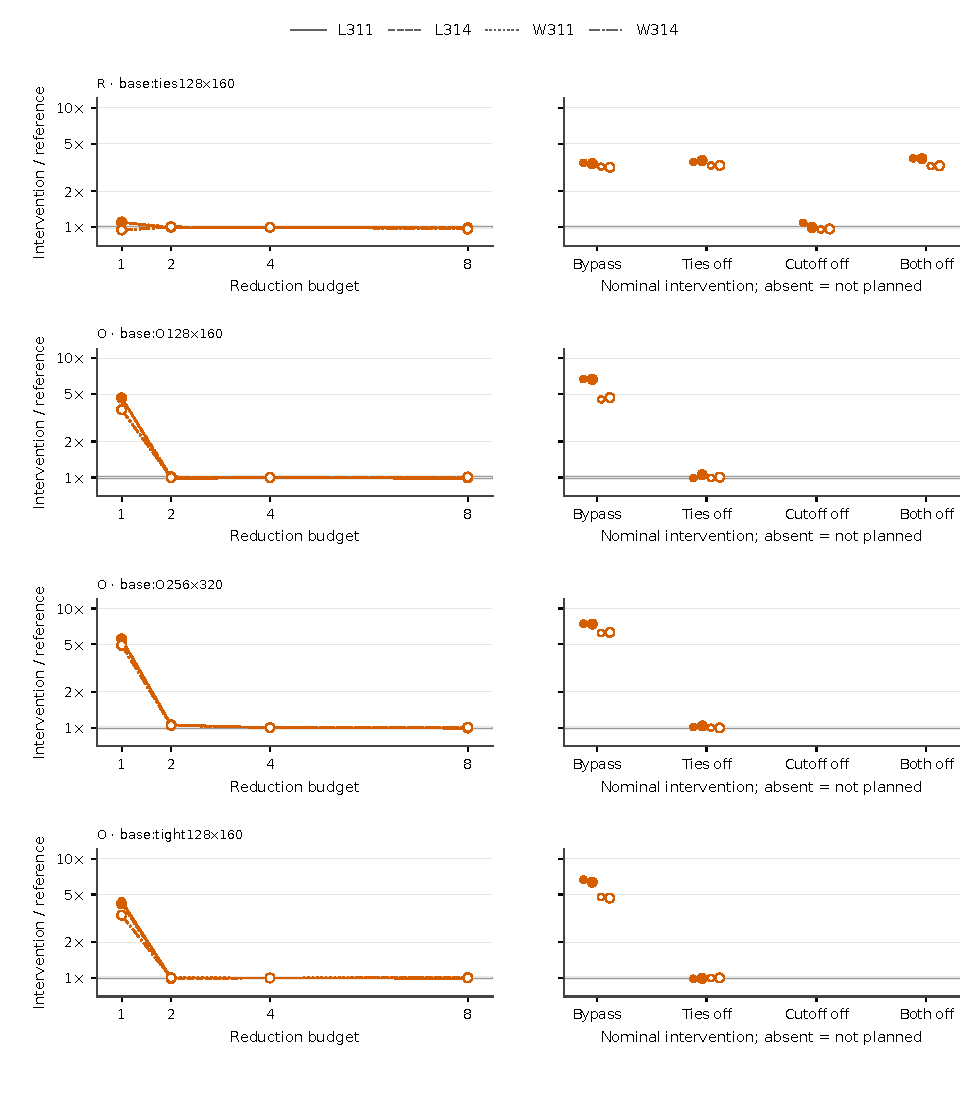
\includegraphics[width=\textwidth,height=.82\textheight,keepaspectratio]{images/current/S_policy_lines_cpp_2.pdf}
\end{center}
\clearpage
\section*{Atlas 31. CPP policy cases, page 3/8}
\noindent One row per workload; R/O mean required/optional. Left: the ordered reduction-budget sweep. Right: independent nominal interventions, drawn only where planned. Every mark/curve is one environment. Ratios are intervention/reference, so above one is slower. Exact case identities and all values remain in the indexed S3 policy timing exports and F5\_budget\_data.csv.
\par\medskip
\begin{center}
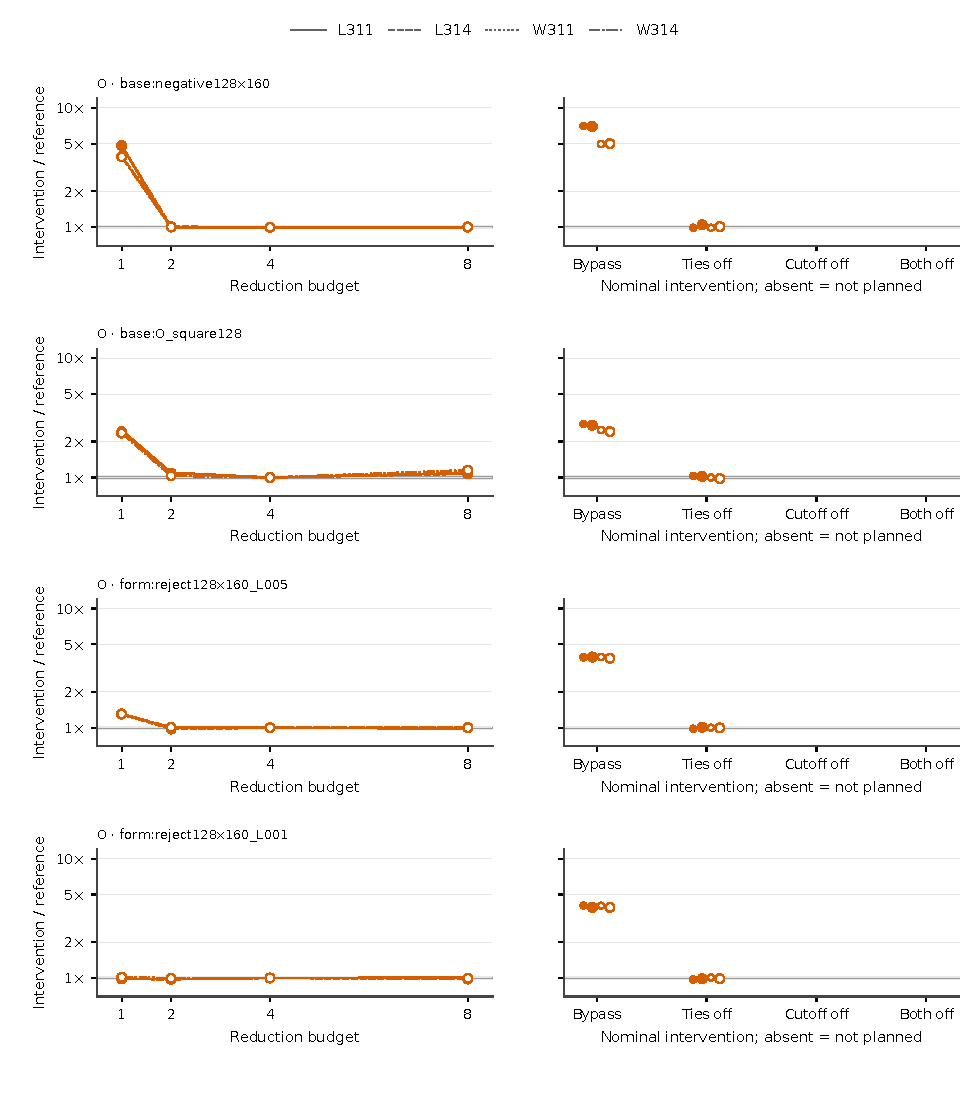
\includegraphics[width=\textwidth,height=.82\textheight,keepaspectratio]{images/current/S_policy_lines_cpp_3.pdf}
\end{center}
\clearpage
\section*{Atlas 32. CPP policy cases, page 4/8}
\noindent One row per workload; R/O mean required/optional. Left: the ordered reduction-budget sweep. Right: independent nominal interventions, drawn only where planned. Every mark/curve is one environment. Ratios are intervention/reference, so above one is slower. Exact case identities and all values remain in the indexed S3 policy timing exports and F5\_budget\_data.csv.
\par\medskip
\begin{center}
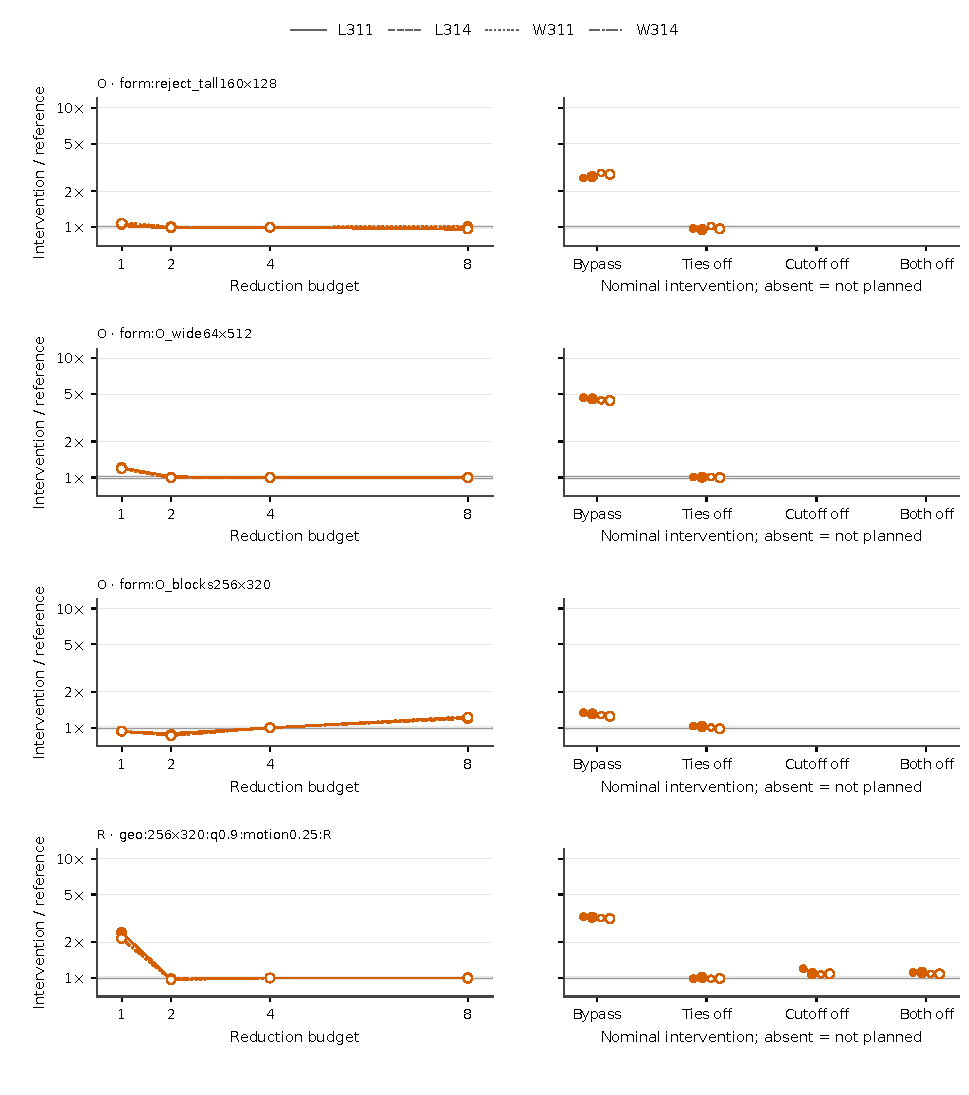
\includegraphics[width=\textwidth,height=.82\textheight,keepaspectratio]{images/current/S_policy_lines_cpp_4.pdf}
\end{center}
\clearpage
\section*{Atlas 33. CPP policy cases, page 5/8}
\noindent One row per workload; R/O mean required/optional. Left: the ordered reduction-budget sweep. Right: independent nominal interventions, drawn only where planned. Every mark/curve is one environment. Ratios are intervention/reference, so above one is slower. Exact case identities and all values remain in the indexed S3 policy timing exports and F5\_budget\_data.csv.
\par\medskip
\begin{center}
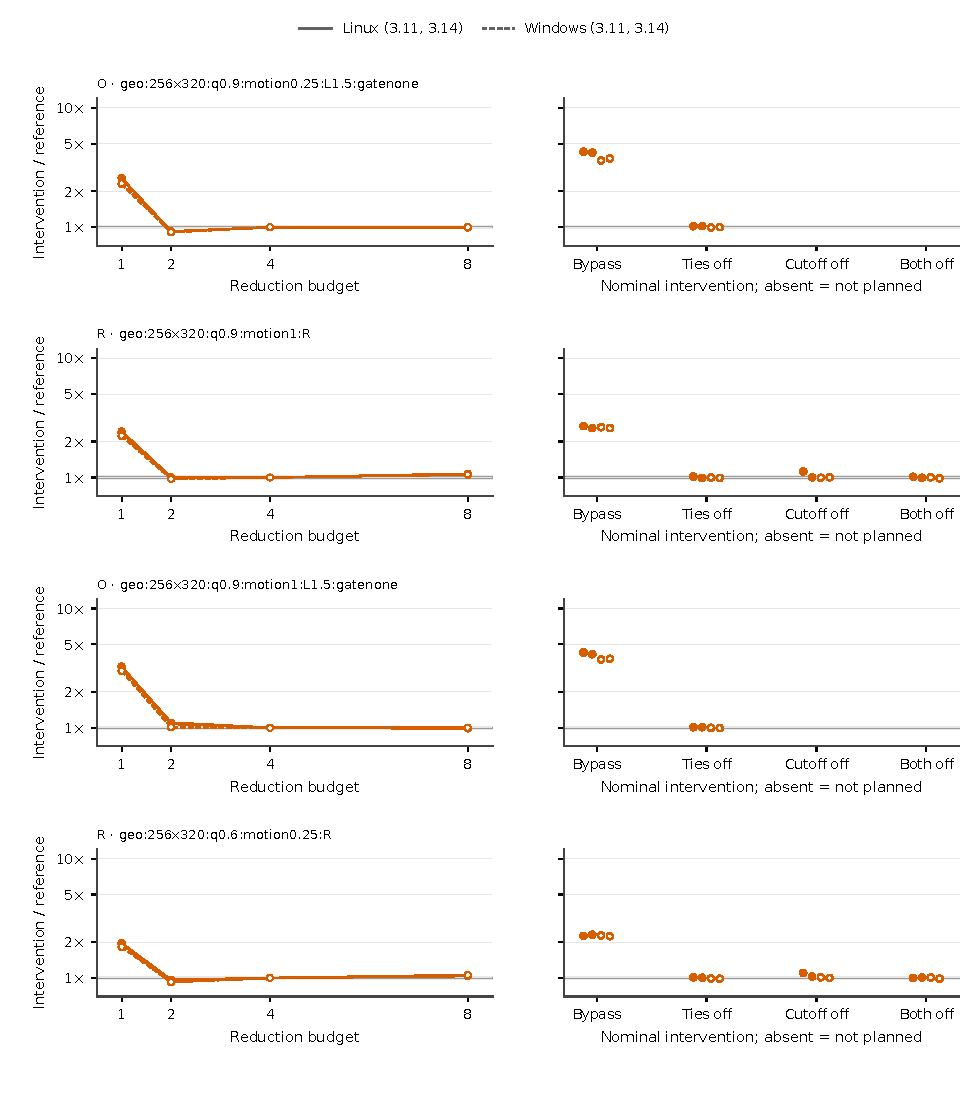
\includegraphics[width=\textwidth,height=.82\textheight,keepaspectratio]{images/current/S_policy_lines_cpp_5.pdf}
\end{center}
\clearpage
\section*{Atlas 34. CPP policy cases, page 6/8}
\noindent One row per workload; R/O mean required/optional. Left: the ordered reduction-budget sweep. Right: independent nominal interventions, drawn only where planned. Every mark/curve is one environment. Ratios are intervention/reference, so above one is slower. Exact case identities and all values remain in the indexed S3 policy timing exports and F5\_budget\_data.csv.
\par\medskip
\begin{center}
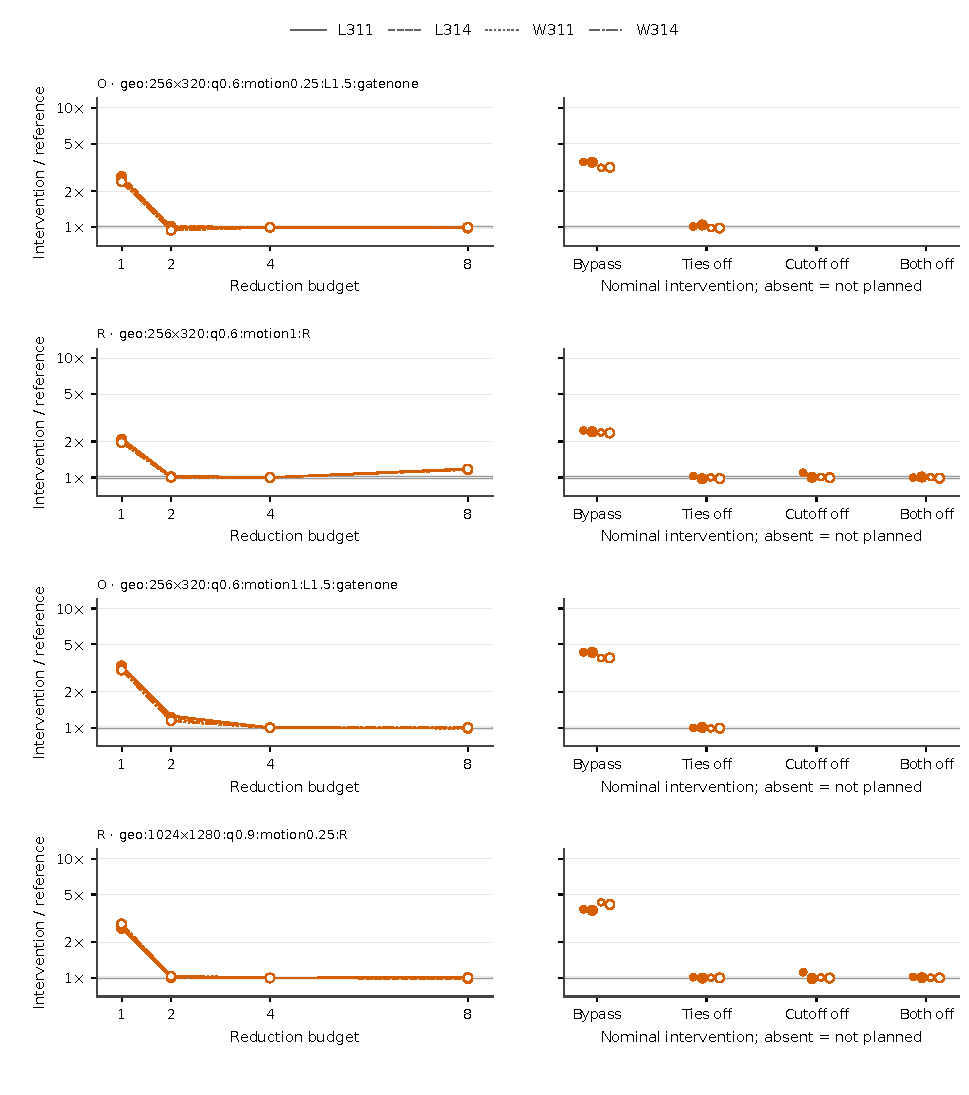
\includegraphics[width=\textwidth,height=.82\textheight,keepaspectratio]{images/current/S_policy_lines_cpp_6.pdf}
\end{center}
\clearpage
\section*{Atlas 35. CPP policy cases, page 7/8}
\noindent One row per workload; R/O mean required/optional. Left: the ordered reduction-budget sweep. Right: independent nominal interventions, drawn only where planned. Every mark/curve is one environment. Ratios are intervention/reference, so above one is slower. Exact case identities and all values remain in the indexed S3 policy timing exports and F5\_budget\_data.csv.
\par\medskip
\begin{center}
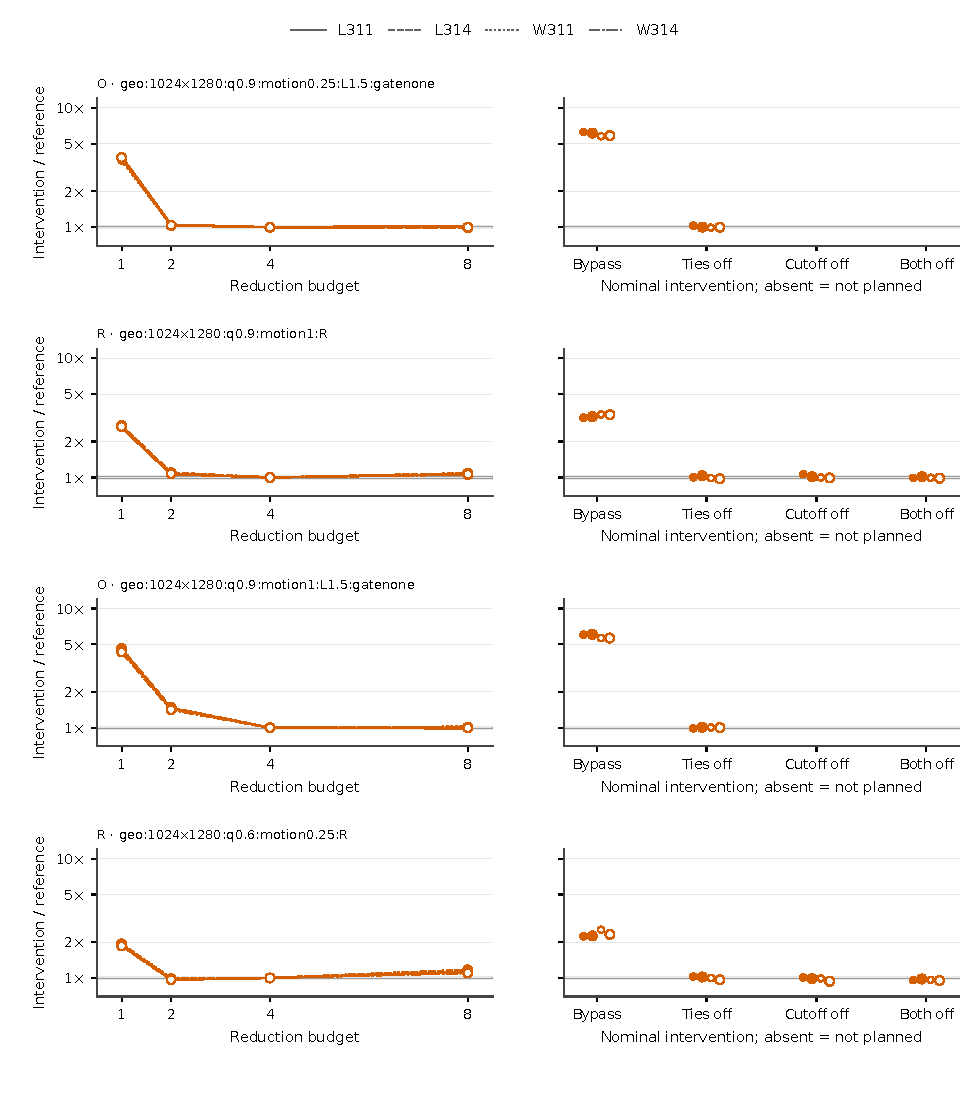
\includegraphics[width=\textwidth,height=.82\textheight,keepaspectratio]{images/current/S_policy_lines_cpp_7.pdf}
\end{center}
\clearpage
\section*{Atlas 36. CPP policy cases, page 8/8}
\noindent One row per workload; R/O mean required/optional. Left: the ordered reduction-budget sweep. Right: independent nominal interventions, drawn only where planned. Every mark/curve is one environment. Ratios are intervention/reference, so above one is slower. Exact case identities and all values remain in the indexed S3 policy timing exports and F5\_budget\_data.csv.
\par\medskip
\begin{center}
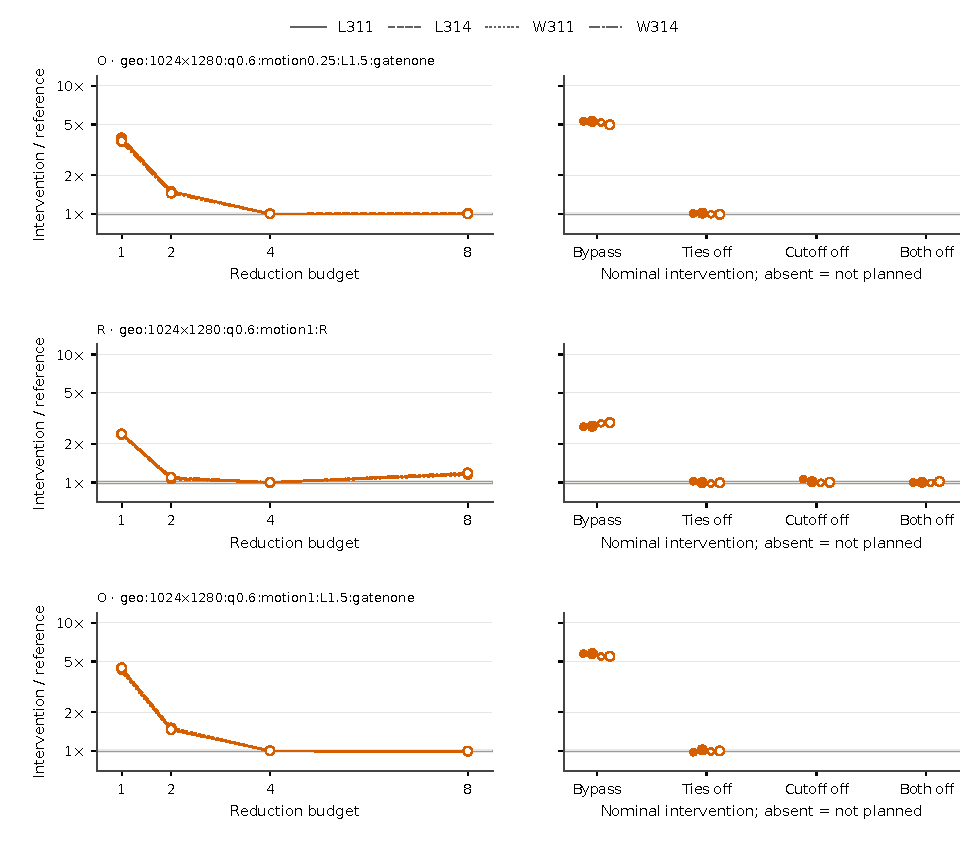
\includegraphics[width=\textwidth,height=.82\textheight,keepaspectratio]{images/current/S_policy_lines_cpp_8.pdf}
\end{center}
\clearpage
\section*{Atlas 37. Shape representations: scipy}
\noindent All 9 eligible workloads per layout. Each marker is one workload/environment. Layouts are categorical and are therefore not connected by lines. Exact case-level values remain in S3\_layout\_timing.csv.
\par\medskip
\begin{center}
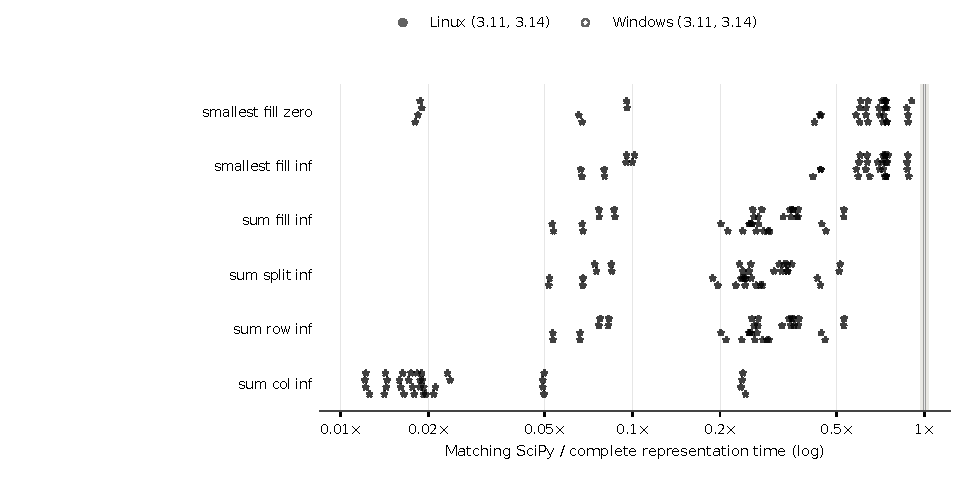
\includegraphics[width=\textwidth,height=.82\textheight,keepaspectratio]{images/current/S_layout_strip_shape_scipy.pdf}
\end{center}
\clearpage
\section*{Atlas 38. Shape representations: jvx}
\noindent All 9 eligible workloads per layout. Each marker is one workload/environment. Layouts are categorical and are therefore not connected by lines. Exact case-level values remain in S3\_layout\_timing.csv.
\par\medskip
\begin{center}
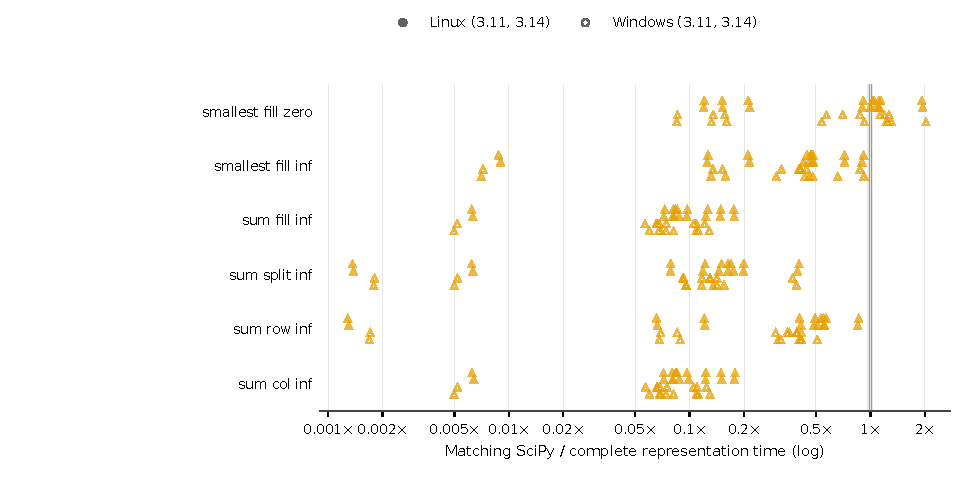
\includegraphics[width=\textwidth,height=.82\textheight,keepaspectratio]{images/current/S_layout_strip_shape_jvx.pdf}
\end{center}
\clearpage
\section*{Atlas 39. Shape representations: jvs}
\noindent All 9 eligible workloads per layout. Each marker is one workload/environment. Layouts are categorical and are therefore not connected by lines. Exact case-level values remain in S3\_layout\_timing.csv.
\par\medskip
\begin{center}
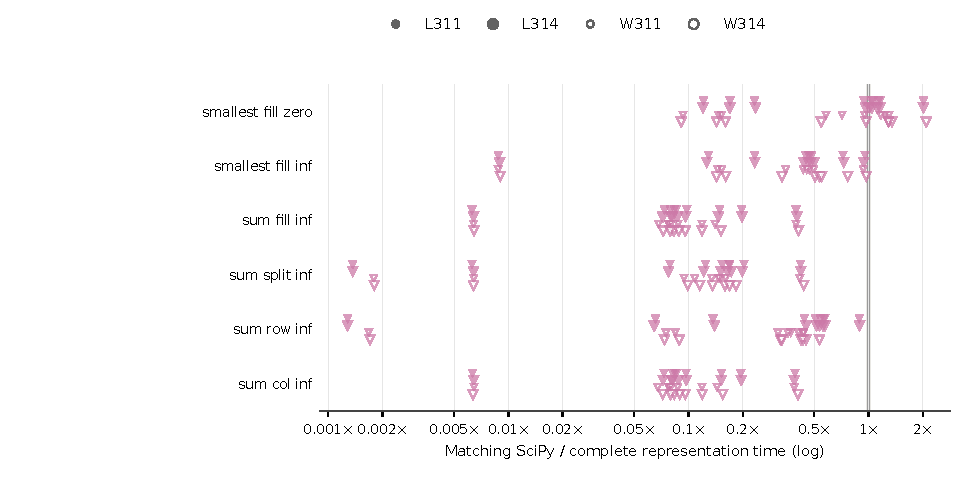
\includegraphics[width=\textwidth,height=.82\textheight,keepaspectratio]{images/current/S_layout_strip_shape_jvs.pdf}
\end{center}
\clearpage
\section*{Atlas 40. Cost representations: scipy}
\noindent All 14 eligible workloads per layout. Each marker is one workload/environment. Layouts are categorical and are therefore not connected by lines. Exact case-level values remain in S3\_layout\_timing.csv.
\par\medskip
\begin{center}
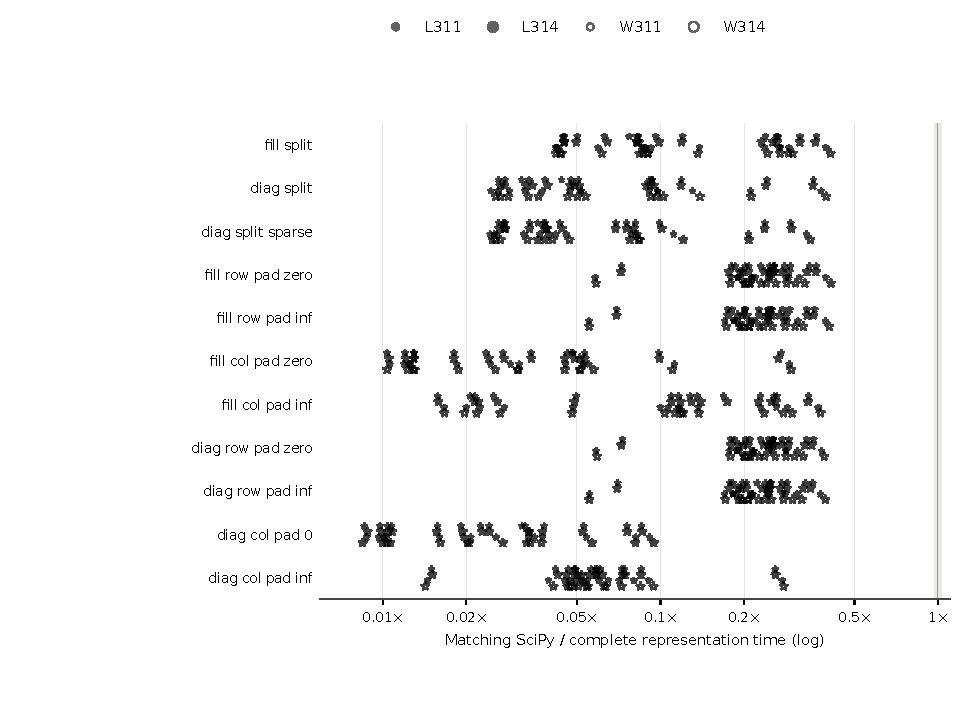
\includegraphics[width=\textwidth,height=.82\textheight,keepaspectratio]{images/current/S_layout_strip_cost_scipy.pdf}
\end{center}
\clearpage
\section*{Atlas 41. Cost representations: jvx}
\noindent All 14 eligible workloads per layout. Each marker is one workload/environment. Layouts are categorical and are therefore not connected by lines. Exact case-level values remain in S3\_layout\_timing.csv.
\par\medskip
\begin{center}
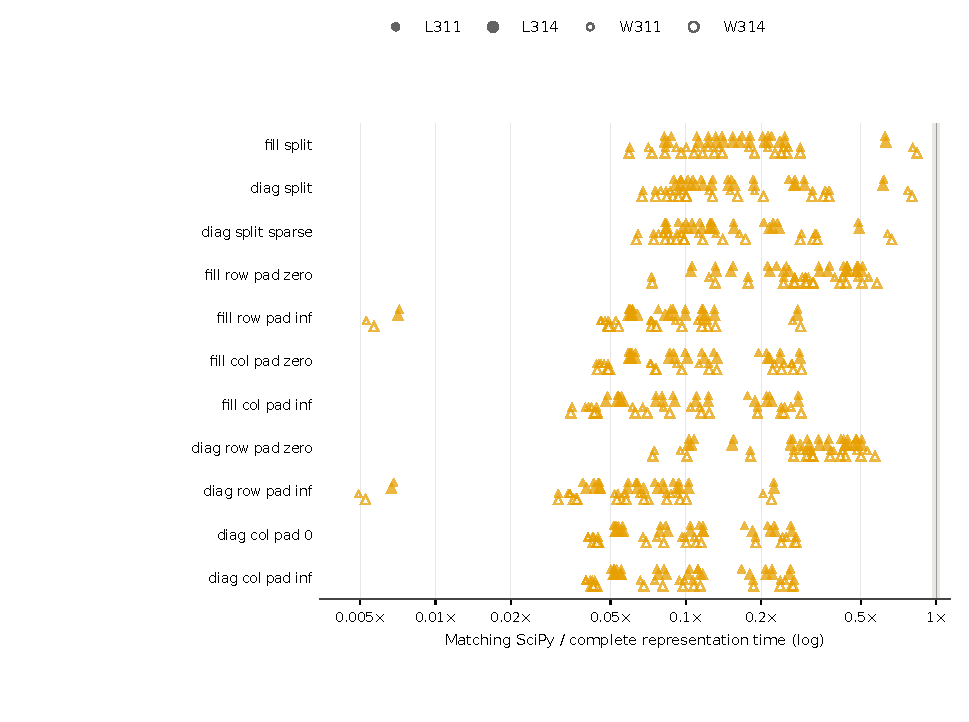
\includegraphics[width=\textwidth,height=.82\textheight,keepaspectratio]{images/current/S_layout_strip_cost_jvx.pdf}
\end{center}
\clearpage
\section*{Atlas 42. Cost representations: jvs}
\noindent All 14 eligible workloads per layout. Each marker is one workload/environment. Layouts are categorical and are therefore not connected by lines. Exact case-level values remain in S3\_layout\_timing.csv.
\par\medskip
\begin{center}
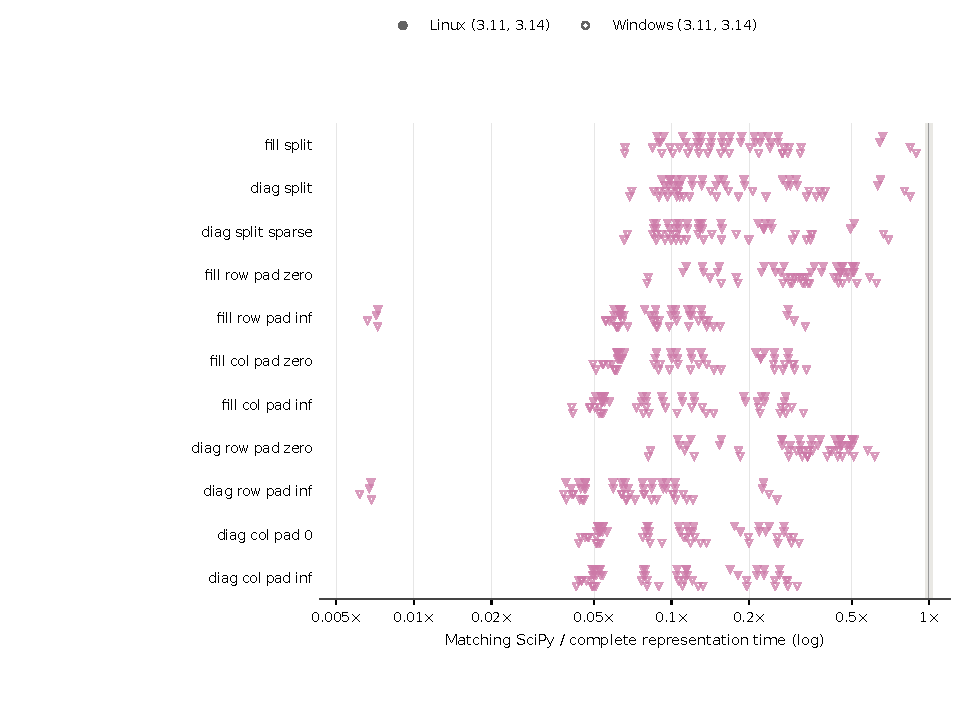
\includegraphics[width=\textwidth,height=.82\textheight,keepaspectratio]{images/current/S_layout_strip_cost_jvs.pdf}
\end{center}
\clearpage
\section*{Atlas 43. Workspace reuse with one worker}
\noindent Each marker is one workload, method and environment. Recreate/retain ratios above one favour retaining state. The main batch figure shows four-worker reuse.
\par\medskip
\begin{center}
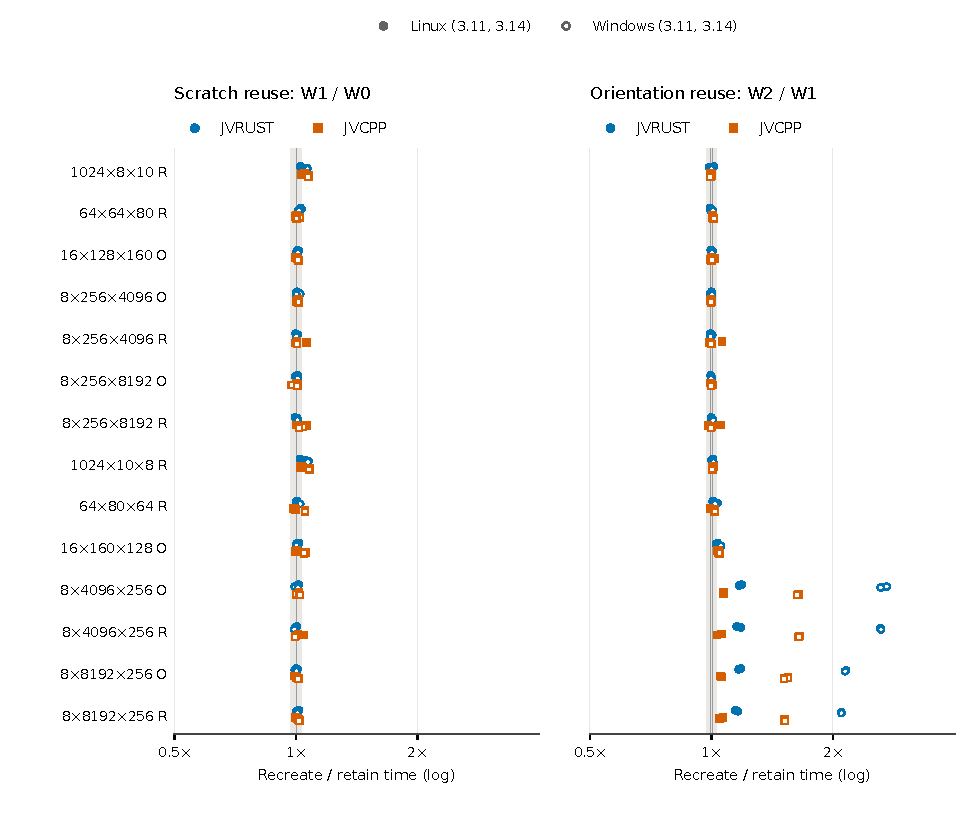
\includegraphics[width=\textwidth,height=.82\textheight,keepaspectratio]{images/current/S_batch_reuse_one_worker.pdf}
\end{center}
\clearpage
% Generated by paper_artifacts_support_figures.py.
\section*{Application API ratios}
Each cell gives float32 assignment replay / tracker.update speed ratios, each relative to SciPy within the same environment. Values are displayed to three decimals; classifications use unrounded values. Absolute times and round estimates remain in S4 exports.
\subsection*{MOT16-04 / GT / Centroid}
\begin{center}\small
\begin{tabular}{lrrrr}
\toprule
API & L311 & L314 & W311 & W314 \\
\midrule
JVRUST & 2.505 / 1.084 & 2.465 / 1.078 & 2.564 / 1.090 & 2.574 / 1.085 \\
JVCPP & 2.515 / 1.083 & 2.478 / 1.077 & 2.380 / 1.084 & 2.398 / 1.083 \\
JVHYBRID & 2.478 / 1.079 & 2.456 / 1.076 & 2.614 / 1.086 & 2.598 / 1.090 \\
JVX row-map & 1.355 / 1.017 & 1.350 / 1.011 & 1.299 / 1.018 & 1.258 / 1.013 \\
JVX indices & 1.411 / 1.027 & 1.405 / 1.013 & 1.367 / 1.022 & 1.319 / 1.021 \\
JVX pairs & 1.574 / 1.041 & 1.543 / 1.033 & 1.519 / 1.042 & 1.491 / 1.029 \\
JVS & 1.547 / 1.031 & 1.572 / 1.018 & 1.484 / 1.023 & 1.321 / 1.028 \\
\bottomrule
\end{tabular}
\end{center}
\subsection*{MOT16-04 / RF-DETR / Centroid}
\begin{center}\small
\begin{tabular}{lrrrr}
\toprule
API & L311 & L314 & W311 & W314 \\
\midrule
JVRUST & 1.935 / 1.072 & 1.917 / 1.067 & 1.992 / 1.078 & 2.013 / 1.072 \\
JVCPP & 1.990 / 1.073 & 1.978 / 1.069 & 1.991 / 1.080 & 2.013 / 1.066 \\
JVHYBRID & 1.904 / 1.073 & 1.886 / 1.060 & 2.012 / 1.082 & 2.022 / 1.073 \\
JVX row-map & 0.714 / 0.928 & 0.711 / 0.925 & 0.752 / 0.942 & 0.732 / 0.930 \\
JVX indices & 0.742 / 0.939 & 0.734 / 0.932 & 0.777 / 0.954 & 0.763 / 0.940 \\
JVX pairs & 0.816 / 0.966 & 0.794 / 0.958 & 0.870 / 0.977 & 0.848 / 0.963 \\
JVS & 0.732 / 0.934 & 0.749 / 0.937 & 0.783 / 0.944 & 0.775 / 0.926 \\
\bottomrule
\end{tabular}
\end{center}
\clearpage
\subsection*{MOT20-03 / GT / Centroid}
\begin{center}\small
\begin{tabular}{lrrrr}
\toprule
API & L311 & L314 & W311 & W314 \\
\midrule
JVRUST & 2.778 / 1.095 & 2.778 / 1.091 & 2.922 / 1.111 & 2.878 / 1.109 \\
JVCPP & 2.809 / 1.096 & 2.807 / 1.095 & 2.654 / 1.107 & 2.699 / 1.108 \\
JVHYBRID & 2.803 / 1.095 & 2.800 / 1.094 & 2.922 / 1.113 & 2.917 / 1.114 \\
JVX row-map & 1.709 / 1.050 & 1.709 / 1.046 & 1.653 / 1.060 & 1.662 / 1.047 \\
JVX indices & 1.736 / 1.054 & 1.737 / 1.048 & 1.731 / 1.059 & 1.700 / 1.055 \\
JVX pairs & 1.810 / 1.061 & 1.800 / 1.058 & 1.819 / 1.068 & 1.780 / 1.067 \\
JVS & 1.929 / 1.061 & 1.957 / 1.056 & 1.887 / 1.069 & 1.859 / 1.062 \\
\bottomrule
\end{tabular}
\end{center}
\subsection*{MOT20-03 / RF-DETR / Centroid}
\begin{center}\small
\begin{tabular}{lrrrr}
\toprule
API & L311 & L314 & W311 & W314 \\
\midrule
JVRUST & 2.136 / 1.078 & 2.109 / 1.077 & 2.229 / 1.087 & 2.168 / 1.086 \\
JVCPP & 2.213 / 1.077 & 2.195 / 1.079 & 2.232 / 1.092 & 2.206 / 1.087 \\
JVHYBRID & 2.098 / 1.071 & 2.060 / 1.075 & 2.263 / 1.091 & 2.229 / 1.078 \\
JVX row-map & 0.663 / 0.923 & 0.658 / 0.918 & 0.783 / 0.953 & 0.760 / 0.946 \\
JVX indices & 0.677 / 0.926 & 0.671 / 0.924 & 0.804 / 0.962 & 0.782 / 0.951 \\
JVX pairs & 0.714 / 0.941 & 0.700 / 0.941 & 0.861 / 0.976 & 0.841 / 0.969 \\
JVS & 0.677 / 0.925 & 0.682 / 0.927 & 0.828 / 0.954 & 0.813 / 0.955 \\
\bottomrule
\end{tabular}
\end{center}
\clearpage
\subsection*{MOT16-04 / GT / Sort}
\begin{center}\small
\begin{tabular}{lrrrr}
\toprule
API & L311 & L314 & W311 & W314 \\
\midrule
JVRUST & 2.427 / 1.005 & 2.389 / 1.005 & 2.524 / 1.004 & 2.492 / 1.000 \\
JVCPP & 2.504 / 1.006 & 2.471 / 1.009 & 2.406 / 1.006 & 2.397 / 1.004 \\
JVHYBRID & 2.400 / 1.005 & 2.384 / 1.006 & 2.561 / 0.997 & 2.519 / 1.005 \\
JVX row-map & 1.354 / 0.999 & 1.350 / 0.999 & 1.312 / 0.996 & 1.248 / 0.993 \\
JVX indices & 1.411 / 1.000 & 1.407 / 0.999 & 1.364 / 1.001 & 1.309 / 0.999 \\
JVX pairs & 1.567 / 1.000 & 1.542 / 1.003 & 1.513 / 1.000 & 1.457 / 0.996 \\
JVS & 1.513 / 1.000 & 1.549 / 1.002 & 1.470 / 1.006 & 1.412 / 0.999 \\
\bottomrule
\end{tabular}
\end{center}
\subsection*{MOT16-04 / RF-DETR / Sort}
\begin{center}\small
\begin{tabular}{lrrrr}
\toprule
API & L311 & L314 & W311 & W314 \\
\midrule
JVRUST & 2.290 / 1.014 & 2.261 / 1.008 & 2.301 / 1.008 & 2.314 / 1.004 \\
JVCPP & 2.329 / 1.015 & 2.316 / 1.008 & 2.280 / 0.998 & 2.287 / 1.005 \\
JVHYBRID & 2.239 / 1.015 & 2.218 / 1.007 & 2.339 / 1.000 & 2.328 / 1.010 \\
JVX row-map & 0.847 / 0.999 & 0.838 / 0.989 & 0.834 / 0.992 & 0.804 / 0.988 \\
JVX indices & 0.880 / 0.998 & 0.873 / 0.989 & 0.860 / 0.993 & 0.837 / 0.991 \\
JVX pairs & 0.970 / 1.002 & 0.952 / 0.992 & 0.965 / 0.995 & 0.947 / 0.990 \\
JVS & 0.866 / 0.999 & 0.891 / 0.992 & 0.865 / 0.994 & 0.845 / 0.992 \\
\bottomrule
\end{tabular}
\end{center}
\clearpage
\subsection*{MOT20-03 / GT / Sort}
\begin{center}\small
\begin{tabular}{lrrrr}
\toprule
API & L311 & L314 & W311 & W314 \\
\midrule
JVRUST & 2.930 / 1.010 & 2.923 / 1.011 & 3.143 / 1.012 & 3.073 / 1.005 \\
JVCPP & 2.990 / 1.012 & 2.976 / 1.011 & 2.919 / 1.009 & 2.908 / 1.009 \\
JVHYBRID & 2.941 / 1.010 & 2.935 / 1.011 & 3.172 / 1.011 & 3.069 / 1.008 \\
JVX row-map & 1.908 / 1.002 & 1.904 / 1.005 & 1.802 / 1.003 & 1.798 / 1.002 \\
JVX indices & 1.946 / 1.006 & 1.944 / 1.006 & 1.911 / 1.007 & 1.834 / 1.001 \\
JVX pairs & 2.039 / 1.007 & 2.021 / 1.008 & 2.007 / 1.008 & 1.921 / 1.003 \\
JVS & 2.147 / 1.007 & 2.175 / 1.008 & 2.094 / 1.006 & 2.017 / 1.002 \\
\bottomrule
\end{tabular}
\end{center}
\subsection*{MOT20-03 / RF-DETR / Sort}
\begin{center}\small
\begin{tabular}{lrrrr}
\toprule
API & L311 & L314 & W311 & W314 \\
\midrule
JVRUST & 2.659 / 1.004 & 2.625 / 1.004 & 2.691 / 0.995 & 2.693 / 1.006 \\
JVCPP & 2.702 / 1.005 & 2.676 / 1.005 & 2.669 / 0.995 & 2.649 / 1.006 \\
JVHYBRID & 2.585 / 1.005 & 2.550 / 1.004 & 2.736 / 1.006 & 2.717 / 1.005 \\
JVX row-map & 1.097 / 0.997 & 1.084 / 0.996 & 1.052 / 0.992 & 1.028 / 0.996 \\
JVX indices & 1.129 / 0.997 & 1.118 / 0.996 & 1.099 / 0.987 & 1.069 / 1.000 \\
JVX pairs & 1.228 / 0.997 & 1.197 / 0.997 & 1.198 / 0.991 & 1.167 / 0.999 \\
JVS & 1.136 / 0.997 & 1.152 / 0.997 & 1.127 / 0.988 & 1.100 / 0.999 \\
\bottomrule
\end{tabular}
\end{center}


\end{document}
